% **************************************************
% Macro specifiche per il documento corrente
% **************************************************
% Nome
\newcommand{\docName}{Norme di Progetto}
% Nome file
\newcommand{\docFileName}{norme\_di\_progetto.3.0.pdf}
% Versione
\newcommand{\docVers}{3.0}
% Data creazione
\newcommand{\creationDate}{2012-12-01}
% Data ultima modifica
\newcommand{\modificationDate}{2013-02-16}
% Stato in {Approvato, Non approvato}
\newcommand{\docState}{Approvato}
% Uso in {Interno, Esterno}
\newcommand{\docUsage}{Interno}
% Destinatari da specificare come nome1\\ &nome2\\ ecc.
\newcommand{\docDistributionList}{Membri del Team}
% Redattori da specificare come nome1\\ &nome2\\ ecc.
\newcommand{\docAuthors}{Riccardo Tresoldi}
% Approvato da
\newcommand{\approvedBy}{Diego Beraldin}
% Verificatori
\newcommand{\verifiedBy}{Andrea Meneghinello}
% Perscorso (relativo o assoluto) che punta alla directory contenente shared/
% come sua sottodirectory (per comodità chiamiamola 'doc root').
\newcommand{\docRoot}{..}
% definire se si vuole l'indice delle tabelle
\def\INDICETABELLE{true}
% definire se si vuole l'indice delle figure
\def\INDICEFIGURE{true}

% importa il preambolo condiviso da tutti i documenti
% shared/preamble.tex
%
% Questo documento contiene la parte del preambolo condivisa e viene pertanto
% richiamato nel 'master' di tutti i documenti di progetto.  Al suo interno
% contiene le inclusioni (e le configurazioni) di tutti i package richiesti per
% la compilazione dei documenti, le macro di carattere generale e la definizione
% degli stili di pagina.

\documentclass[a4paper,10pt,openright]{article}

% **************************************************
% Macro generiche
% **************************************************
\newcommand{\team}{Software Synthesis}                    % chi siamo
\newcommand{\email}{software.synthesis@gmail.com}         % e-mail
\newcommand{\caName}{}                                    % titolo capitolato
\newcommand{\caDescr}{}                                   % descrizione
\newcommand{\inglese}[1]{\textit{#1}}

% **************************************************
% Codifica e lingua dei documenti
% **************************************************
\usepackage[utf8x]{inputenc}                              % codifica caratteri dei documenti sorgenti
\usepackage[english,italian]{babel}                       % localizzazione ai fini di sillabazione e cross-references
\usepackage[T1]{fontenc}                                  % codifica font di output

% **************************************************
% Definizione geometria della pagina
% **************************************************
\usepackage[a4paper,head=4cm,top=4.5cm,bottom=3cm,left=3cm,right=3cm,bindingoffset=5mm]{geometry}

% *************************************************
% Intestazioni e piè di pagina personalizzati
% *************************************************
\usepackage{fancyhdr}
% stile normale
\fancypagestyle{normal}{
\fancyhead{}                                              % intestazione
\fancyhead[RE,RO]{
\begin{picture}(0,0)
  \put(-410,0){
\includegraphics[width=1.02\textwidth]{header_logo}}
  \put(-410,10){\sffamily\large\leftmark}
\end{picture}
\vspace{-4pt}
}
\renewcommand{\headrulewidth}{.4pt}                       % riga sotto l'intestazione
\cfoot{}                                                  % piè di pagina
\fancyfoot[RO,LE]{\sffamily
  pag.~\thepage{} di \pageref{LastPage}}                  % a dx nelle pag. dispari e a sx in quelle pari
\fancyfoot[RE,LO]{\sffamily\docFileName{} -- v.\docVers}
\renewcommand{\footrulewidth}{.4pt}                       % riga sopra il piè di pagina
}
% stile per gli indici
\fancypagestyle{toc}{
\fancyhead{}                                              % intestazione
\fancyhead[RE,RO]{
\begin{picture}(0,0)
  \put(-410,0){
\includegraphics[width=1.02\textwidth]{header_logo}}
\end{picture}
}
\renewcommand{\headrule}{}                                % nessuna riga sotto l'intestazione
\cfoot{}                                                  % piè di pagina
\fancyfoot[RO,LE]{\sffamily\thepage{}}                    % a dx nelle pag. dispari e a sx in quelle pari
\fancyfoot[RE,LO]{\sffamily\docFileName{} -- v.\docVers}
\renewcommand{\footrulewidth}{.4pt}                       % riga sopra il piè di pagina
}

\pagestyle{fancy}                                         % premetto: non so usare bene le marche:
\renewcommand{\sectionmark}[1]{\markboth{#1}{#1}}         % se qualcuno ha idee migliori si faccia avanti!

% **************************************************
% Tabelle
% **************************************************
\usepackage{tabularx}                                     % tabelle di larghezza fissa con una o più colonne variabili
\usepackage{multirow}                                     % colonne con colonne che si estendono per più righe
\usepackage{booktabs}                                     % per inserire l'ambiente table e le righe orizz. nelle tabelle
\usepackage{longtable}			                          % tabelle oltre i limiti di pagina

% **************************************************
% Cross-references e collegamenti ipertestuali
% **************************************************
\usepackage[hidelinks]{hyperref}
\hypersetup{%
  colorlinks=false, linktocpage=false, pdfborder={0,0,0}, pdfstartpage=3, pdfstartview=FitV,%
  urlcolor=Cyan, linkcolor=Cyan, citecolor=Black, %pagecolor=Black,%
  pdftitle={\docName}, pdfauthor={\team}, pdfsubject={}, pdfkeywords={},%
  pdfcreator={pdflatex}, pdfproducer={pdflatex with hyperref package}%
}

% **************************************************
% Immagini e grafica
% **************************************************
\usepackage{graphicx}                                     % supporto ad aspetti avanzati delle immagini
\graphicspath{{\docRoot/pics/}}                           % percorso contenente tutti i file immagini
\usepackage{color}                                        % permette di colorare facilmente il testo

% **************************************************
% Altri pacchetti opzionali
% **************************************************     
\usepackage{lastpage}                                     % per sapere il numero totale di pagine
\usepackage{lipsum}                                       % genera "dummy text" per prove di impaginazione
\usepackage{eurosym}                                      % per il simbolo dell'euro usare \EUR{x} dove x è l'importo


% Fine del preambolo e inizio del documento
\begin{document}

% Inclusione della prima pagina
% shared/firstpage.tex
%
% Questo documento definisce il contenuto della prima pagina, che si suppone
% essere uguale in tutti i documenti.  Oltre al logo e al titolo, la prima
% pagina contiene i metadati relativi al documento in cui viene inclusa.


% rimuove intestazioni e piè di pagina
\pagestyle{empty}

\begin{center}

% logo del gruppo

\includegraphics[width=1.5\textwidth]{logo}

\vspace{1in}

% titolo del documento
{\Huge\bfseries \docName}

\vspace{1in}

% tabella riepilogativa
\begin{tabularx}{.7\textwidth}{>{\bfseries\sffamily}l>{\sffamily}l}
\toprule
\multicolumn{2}{>{\sffamily}c}{Informazioni sul documento}\\
\midrule
Nome file:            & \docFileName\\
Versione:             & \docVers\\
Data creazione:       & \creationDate\\
Data ultima modifica: & \modificationDate\\
Stato:                & \docState\\
Uso:                  & \docUsage\\
Redattori:            & \docAuthors\\
Approvato da:         & \approvedBy\\
Verificatori:         & \verifiedBy\\
\bottomrule
\end{tabularx}

\end{center}

\newpage


% Storico delle modifiche
\section*{Storia delle modifiche}
\begin{tabularx}{\textwidth}{lXlll}
\toprule
Versione & Descrizione intervento & Membro & Ruolo & Data\\
\midrule % inserire qui il contenuto della tabella


3.0 & Approvazione documento & Diego Beraldin & Responsabile & 2013-02-16\\
2.7 & Correzione lessico ortografica del documento & Andrea Meneghinello & Verificatore & 2013-02-14\\
2.6 & Rese le sezioni del documento più procedurali & Riccardo Tresoldi & Amministratore & 2013-02-14\\
2.5 & Aggiunta e redatta sezione test & Riccardo Tresoldi & Amministratore & 2013-02-14\\
2.4 & Correzione e aggiornamento sezione strumenti & Riccardo Tresoldi & Amministratore & 2013-02-12\\
2.3 & Correzione e aggiornamento sezione verifica & Riccardo Tresoldi & Amministratore & 2013-02-11\\
2.2 & Aggiunta e redatta sezione Progettazione di dettaglio e Rapporti intrapersonali & Riccardo Tresoldi & Amministratore & 2013-02-11\\
2.1 & Aggiunta nota sulla rotazione dei redattori & Riccardo Tresoldi & Amministratore & 2013-02-08\\
2.0 & Approvazione documento & Riccardo Tresoldi & Responsabile & 2013-01-23\\
1.6 & Correzione errori rilevati dal verificatore & Diego Beraldin & Amministratore & 2013-01-22\\
1.5 & Validazione del documento & Stefano Farronato & Verificatore & 2013-01-22\\
1.4 & Aggiornata sezione software di tracciamento e verifica & Diego Beraldin & Amministratore & 2013-01-17\\
1.3 & Conclusa sezione progettazione & Diego Beraldin & Amministratore & 2013-01-16\\
1.2 & Aggiunta sezione progettazione & Diego Beraldin & Amministratore & 2013-01-15\\
1.1 & Correzione errori rilevati in RR & Diego Beraldin & Amministratore & 2013-01-12\\
1.0 & Approvazione documento & Stefano Farronato & Responsabile & 2012-12-04\\
0.6 & Validazione documento & Marco Schivo & Verificatore & 2012-12-04\\
0.5 & Fine stesura documento & Andrea Meneghinello & Amministratore & 2012-12-03\\
0.4 & Stesura sezione Milestones e Ticketing, Analisi dei requisiti & Andrea Meneghinello & Amministratore & 2012-12-03\\
0.3 & Stesura sezione ambiente documentale & Andrea Meneghinello & Amministratore & 2012-12-03\\
0.2 & Stesura sezione ambiente di lavoro & Andrea Meneghinello & Amministratore & 2012-12-01\\
0.1 & Stesura scheletro documento, sezione comunicazione & Andrea Meneghinello & Amministratore & 2012-12-01\\
\bottomrule
\end{tabularx}
\clearpage

% inclusione dell'indice
% shared/toc.tex
%
% Questo file contiene le istruzioni che generano l'indice o gli indici del
% documento (utile nel caso in cui decidessimo di avere anche un indice delle
% tabelle e/o un indice delle figure).

\pagestyle{toc}
\pagenumbering{roman}

\tableofcontents

\newpage


% Alcuni aggiustamenti per le pagine
\pagenumbering{arabic}
\setcounter{page}{1}
\pagestyle{normal}

\clearpage
\section{Introduzione}
\subsection{Scopo del prodotto}
\purpose

\subsection{Scopo del documento}
Questo documento viene redatto per definire le norme da adottare da parte di tutti i componenti del gruppo \team{} durante il periodo di svolgimento del capitolato \caName, commissionato dall'azienda Zucchetti S.r.l. In particolare si andranno a definire le regole per:
\begin{itemize}
\item Relazioni interpersonali e comunicazione
\item Definizione dell'ambiente di lavoro
\item Redazione documenti
\item Convenzioni e norme per l'analisi e la progettazione
\item Convenzioni e norme per la verifica di file e documenti
\end{itemize}

\subsection{Ambiguità}
Al fine di evitare incomprensioni dovute all'uso di termini tecnici nei documenti, viene redatto e allegato il documento \textit{glossario.3.0.pdf} dove vengono definiti e descritti tutti i termini marcati con una sottolineatura.
\clearpage

\section{Comunicazioni e relazioni intrapersonali}
\subsection{Comunicazione interna}
\label{sec:comunicazione_interna}
La comunicazione tra i vari componenti del team avverrà principalmente durante gli incontri che si terranno in un luogo fisico comune. Per evitare problemi dovuti alla mancata presenza da parte di un membro, le notifiche dell'attività svolta durante l'incontro verranno scritte in un calendario comune messo a disposizione.

Nei casi in cui il lavoro si svolgesse presso la propria abitazione, si potrà utilizzare \textit{Skype} per avviare chat, chiamate e videoconferenze di gruppo.

Qualora si evinca la necessità di un ritrovo fisico comune ma vi fosse l'impossibilità da parte di alcuni membri di recarsi nel luogo prefissato, allora si procederà suddividendo il gruppo in due sottogruppi, ciascuno con un luogo di ritrovo prefissato. I due team di sviluppo quindi potranno comunicare con l'altro team mediante il software di comunicazione prestabilito.


\subsection{Comunicazione esterna}
I contatti verso l'esterno saranno a cura del responsabile di progetto. A tale scopo è stato creato un indirizzo di posta elettronica tramite il quale la persona incaricata tratterà a nome dell'intero gruppo \team{}

L'email sopra descritta è \textit{info@softwaresynthesis.org} e l'inoltro di risposte a tutti gli altri membri sarà sempre a carico del responsabile di progetto che dovrà utilizzare i metodi descritti nella sezione \ref{sec:comunicazione_interna}.

\subsection{Incontri Interni}
Saranno fissate delle riunioni formali decise dal responsabile di progetto che provvederà rendere noto a tutti luogo, data e ora della seduta mediante email personale con almeno tre giorni di anticipo.

Nell'email sarà contenuta anche la motivazione per cui si è reso necessario l'incontro. Ai membri è richiesta la conferma di partecipazione tramite risposta, sempre via email. Nel caso in cui un componente del team non potesse essere presente alla riunione decisa, dovrà specificarne il motivo nell'email di risposta al responsabile.

Ogni membro del gruppo ha la possibilità di richiedere un incontro interno: tale domanda dovrà venir indirizzata sempre al responsabile di progetto, il quale la visionerà e pianificherà un eventuale incontro.

Ad ogni riunione verrà redatto inoltre un verbale in cui verranno annotate tutte le decisioni prese e i punti salienti della discussione.

\subsection{Incontri Esterni}
Sarà il responsabile di progetto a prendere accordi per incontri con il committente o con i proponenti.

Ogni membro del gruppo può richiedere un incontro esterno al responsabile, presentando una motivazione. Questa necessità verrà presentata all'intero team e solo nel momento in cui ci saranno tre conferme, con relativa presenza all'incontro, il responsabile provvederà a prendere appuntamento con la parte esterna. In caso contrario la proposta sarà bocciata.

\subsection{Considerazioni sui rapporti interpersonali}

In questa sotto-sezione si intende riassumere i punti focali inerenti i rapporti tra i membri del team. Tali sono da intendere come suggerimenti da rispettare per il rispetto comune, al fine di non far insorgere litigi controproducenti allo sforzo comune.

\begin{itemize}
	\item \textbf{Usare un linguaggio consono e rispettoso}: si invitano tutti i membri del team ad assumere un comportamento rispettoso verso il prossimo. Con ciò si fa riferimento all'uso di un linguaggio e gestualità civile (anche in virtù del fatto che molti luoghi di riunione sono pubblici).
	\item \textbf{Nessuno è superiore agli altri}: è evidente che tutti i membri del team hanno la medesima esperienza nel campo dell'ingegneria del software (da intendersi sia come conoscenze generali che come grado di ``maturità'' nel settore).
	
Pertanto in ogni dibattito  è richiesto ad ogni membro del team di ricordare che le idee altrui non sono da criticare a prescindere, ma bensì vanno valutate e giudicate coscientemente, dando luogo ad un dibattito nel rispetto di ogni membro del team.
	\item \textbf{Mai mettere alla berlina chi sbaglia}: indubbiamente ogni membro del team, ha delle responsabilità che cambiano in virtù del ruolo che ricopre. Va però ricordato che in caso d'errore non si dovrà giudicare colpevole e conseguentemente screditare un componente del gruppo.
	
Ciò potrebbe si portare chi ha sbagliato a prestare una maggiore attenzione al proprio operato, ma il rischio di  portare il suddetto membro del gruppo a non esporre le proprie idee per pregiudizi su quanto accaduto potrebbe nuocere alla qualità del prodotto finale.

Sarà quindi esclusiva responsabilità del responsabile comunicare in privato gli errori ai relativi ``colpevoli''. Cosi facendo il soggetto sarà corretto e si eviterà che questi si senta pubblicamente umiliato.
\end{itemize}

\clearpage
\section{Ambiente di lavoro}
\subsection{Repository}
\label{sec:repository}
Per un corretto svolgimento del progetto si è reso necessario adottare un luogo dove poter cercare e salvare tutti i documenti da redigere, nonché i file di codifica. Per questo si è deciso di adottare un \underline{\inglese{repository}} ospitato da \inglese{GitHub}.

Il motivo principale di questa scelta sta nel fatto che \texttt{git}, rispetto ad altri sistemi quali \inglese{Sourceforge} ad esempio, è un \underline{sistema di controllo di versione} distribuito.

Rientra infatti nei \inglese{repository} di tipo \inglese{Distribuited Control Version System} (DVCS) mentre \inglese{Sourceforge} rientra nei \inglese{repository} di tipo \inglese{Centralized Control Version System}.

La differenza sta nel fatto che in \texttt{git} ognuno avrà in locale l'intera copia del \inglese{repository}, quindi tutti i vari \inglese{commit}, rami ecc. mentre con \inglese{Sourceforge} in locale si ha solo la situazione dell'ultimo \inglese{commit} e se si deve eseguire operazioni di \inglese{rollback} si ha bisogno della connessione di rete per potersi connettere al \underline{server} centrale.

\subsubsection{Registrazione}
Per utilizzare \inglese{GitHub} occorre registrasi presso:
\begin{center}
\url{https://github.com}.
\end{center}
per far ciò basta inserire un \inglese{username}, un indirizzo \inglese{email} e una \inglese{password} nell'apposito \underline{form} proposto nella pagina sopra indicata.

\subsubsection{Installazione}
Per aiutare i componenti del gruppo nella fase di installazione di \texttt{git}, è stata creata appositamente una guida che passo passo spiega come installare e configurare nel modo giusto il software.\footnote{%
La guida è reperibile all'indirizzo 
\url{https://github.com/SoftwareSynthesis/SoftwareEngineeringProject/blob/master/Manuals/GuidaGit/MasterDocument.pdf}.
}

\subsubsection{Struttura}
\label{sec:struttura}
\begin{itemize}
\item \textbf{Progetto}: l'indirizzo web a cui fa riferimento l'intero progetto è: 
\begin{center}
\url{https://github.com/SoftwareSynthesis/SoftwareEngineeringProject}
\end{center} 
\item \textbf{Documentazione}: tutti i documenti saranno reperibili all'indirizzo
\begin{center}
\url{https://github.com/SoftwareSynthesis/SoftwareEngineeringProject/Documents}
\end{center}
Ogni documento redatto dovrà essere contenuto in una sotto-cartella della directory \verb+Documents+ nominata come il nome del documento stesso: questa conterrà i file \LaTeX.

È inoltre presente una cartella \verb+Revisioni+, composta a sua volta da quattro sotto-cartelle (\verb+RR+, \verb+RP+, \verb+RQ+, \verb+RA+) che conterranno i documenti formali consegnati alle quattro revisioni del progetto ed una cartella \verb+pics+ che conterrà tutte le immagine utilizzate nei documenti.
\item \textbf{Codice}: tutti i file sorgente saranno reperibili all'indirizzo
\begin{center}
\url{https://github.com/SoftwareSynthesis/SoftwareEngineeringProject/Code}
\end{center}
Le regole da adottare per utilizzare questa cartella saranno redatte non appena si verificherà la necessità.
\item \textbf{Others}: per qualsiasi altro file di utilità per il progetto, è stata predisposta una cartella \verb+Others+ utilizzabile da tutti i membri.
\end{itemize}

\subsubsection{Sistema di versionamento}
Come sistema di controllo di versione  è stato adottato \textit{git}. Questo scelta è stata decisa dopo aver individuato diversi pregi, tra i quali:
\begin{itemize}
\item velocità;
\item design semplice;
\item forte supporto allo sviluppo non-lineare (possibilità di migliaia di rami paralleli);
\item completamente distribuito;
\item capacità di gestire, in modo efficiente (velocità e dimensione dei dati), grandi progetti come il kernel Linux.
\end{itemize}

\subsection{Sistema di tracciamento dei requisiti}
\label{sec:tracciamento}
Al fine di rendere automatico e sistematico la gestione del tracciamento dei requisiti, è stato creato un sistema che si appoggia al sito aziendale. Il gestionale è stato nominato ``\manager{}''. Ogni volta che un membro del gruppo necessita di interagire con tale sistema, si dovrà autenticare alla pagina

\begin{center}
\url{http://www.softwaresynthesis.org/Login.php}
\end{center}

Il sistema di tracciamento offre le seguenti 5 opzioni:
\begin{itemize}
\item \textbf{Gestione requisiti}: permette l'inserimento, modifica e la cancellazione di un requisito;
\item \textbf{Gestione fonti}: permette l'inserimento, modifica e la cancellazione di una fonte da intendersi come ad esempio il capitolato d'appalto;
\item \textbf{Gestione casi d'uso}: permette l'inserimento di un caso d'uso con relativi scenari  e requisiti associati;
\item \textbf{Gestione attori}: permette l'inserimento, modifica e la cancellazione di un attore utilizzabile in seguito per lo sviluppo di un caso d'uso;
\item \textbf{Gestione classi}: permette l'inserimento e la cancellazione di una classe rilevata nell'attività di progettazione;
\item \textbf{Gestione componenti}: permette l'inserimento e la cancellazione di una componente rilevata nell'attività di progettazione;
\item \textbf{Gestione design pattern}: permette l'inserimento e la cancellazione di un design pattern utilizzato nel progetto;

\item \textbf{Stampa}: è suddivisa in due sezioni, la prima per la parte di analisi, la seconda per la parte di progettazione.

Il comportamento delle due stampe è analogo, crea in modo automatico un file di estensione .tex contenente nel primo caso la lista dei requisiti analizzati, i casi d'uso studiati e il tracciamento tra i requisiti-casi d'uso e viceversa, nel secondo caso viene stampato la lista di tracciamenti tra classi-componenti-design pattern (vedi sezione \ref{sec:tracciamenti_progettazione}). Successivamente alla stampa tale file sarà da includere all'intero del documento ``\textit{analisi\_dei\_requisiti.tex}'' o ``\textit{specifica\_tecnica.tex}'' a seconda.
\end{itemize}

Il sistema è basato su tecnologie \underline{MySQL} con creazione del \underline{database} sotto engine\_inno\_db . Per sopperire ad alcune mancanze del sistema di tracciamento, lo sviluppatore si potrà appoggiare alla piattaforma \underline{phpMyAdmin} fornita dal \underline{web host}, al fine di modificare e gestire alcuni dati del database.

In particolare, se ne obbliga l'utilizzo nei seguenti casi:
\begin{itemize}
\item modifica di un caso d'uso;
\item cancellazione di un caso d'uso.
\end{itemize}

Quest'obbligo di gestione è dovuto a mancanze temporali nella fase di sviluppo del sistema, nel periodo antecedente alla consegna dei capitolati, e anche in parte per la complessità di implementazione.

Ogni altra modifica attuata tramite \inglese{phpmyadmin} è assolutamente vietata per mansioni che non siano riportate al punto precedente.


\subsection{Sistema operativo}
L'intero progetto verrà portato avanti attraverso sistemi Unix e Windows, più in particolare Mac OSX 10.8.2, Fedora 17, Windows 7, Windows 8. Questa scelta deriva dal fatto che, essendo il progetto \caName{} un applicativo web, non si sono riscontrate dipendenze alcune da librerie di sistema.

\subsection{Diagrammi UML}
Per la produzione di diagrammi UML si adotterà il software ConceptDraw. Questo scelta è stata fatta perchè il \inglese{tool} si presenta molto semplice da usare, è molto potente e permette la creazione di moltissimi diagrammi UML adottando lo standard 2.0.

La qualità dei diagrammi prodotti inoltre è molto buona e le modalità con cui tali diagrammi verranno inseriti sono descritte nella sezione \ref{image}.


\subsection{Diagrammi di Gantt}
Come supporto alla pianificazione del progetto si è scelto di utilizzare Project Libre nella versione 1.5.2, software molto leggero e facile da installare. È uno strumento \inglese{opensource} e multi piattaforma. Permette la creazione di diagrammi di Gantt in modo molto semplice con possibilità di esportarli in formato jpg.

Per il download e l'installazione si rimanda al seguente link:
\begin{center}
\url{http://sourceforge.net/projects/projectlibre/}.
\end{center}
\clearpage

\section{Ambiente documentale}
\label{sec:ambiente_documentale}
In questa sezione verranno illustrati i vari standard utilizzati dal team per la produzione di documenti durante l'intero progetto. 

\subsection{Software utilizzati}
Tutti i documenti dovranno essere scritti in italiano con \LaTeX, un software free di composizione testuale che comprende una serie di caratteristiche atte alla produzione di documentazione tecnica e scientifica.


Per attuare questa scelta, l'azienda \team{} ha deciso di utilizzare come editor \LaTeX{} \textit{TexMaker}, software disponibile sia per ambienti Unix che Windows. Si presenta come un software molto flessibile che include al suo interno la correzione ortografica automatica, l'autocompletamento e un visualizzatore di PDF integrato.

La versione da utilizzare è l'ultima disponibile in tale momento ed è la 3.5.2. Per il download seguire il seguente link:
\begin{center}
\url{http://www.xm1math.net/texmaker/download.html}.
\end{center}
Per l'installazione, una volta scaricato, basta seguire le indicazioni presenti nel file scaricato precedentemente.

\subsection{Nomi dei documenti}
\label{sec:nomi_documenti}
Il nome dei documenti dovrà rappresentare in modo univoco la natura del file e sarà composto nel seguente modo:
\begin{center}
nome\textunderscore del\textunderscore file.X.Y.estensione
\end{center}
dove:
\begin{itemize}
\item \textbf{nome\textunderscore del\textunderscore file}: il nome del file non dovrà contenere lettere maiuscole ne caratteri speciali (compresi accenti). Nel caso sia composto da più parole, questa vanno separate con il carattere ``\inglese{underscore}''.
\item \textbf{Variabile X}: Indica il raggiungimento di uno stato formale rispetto ad una \underline{Milestone}. Assumerà quindi principalmente 4 valori, dall'1 al 4, attribuiti come segue:
\begin{table}[h]
\centering
\rowcolors{2}{lightblue}{llightblue}
\begin{tabular}{ll}
\toprule
Milestone & X\\
\midrule
Revisione dei Requisiti (RR) & 1\\
Revisione dei Requisiti (RP) & 2\\
Revisione dei Requisiti (RQ) & 3\\
Revisione dei Requisiti (RA) & 4\\
\bottomrule
\end{tabular}
\caption{Revisioni e Milestones}
\end{table}
\item \textbf{Variabile Y}: parte dal valore 0 e viene incrementata ogni qualvolta, senza limite superiore, si apportano modifiche sostanziali al documento, come ad esempio la stesura di una nuova sezione o correzione di errori.
\end{itemize}

\subsection{Impostazioni di base di un documento}
Ogni documento dovrà attenersi alle seguenti regole per la sua redazione:
\begin{itemize}
\item \textbf{Intestazione}: composta dalla sezione del documento nella parte sinistra e dal logo nella parte destra.
\item \textbf{Piè di pagina}: composto dal nome del documento con relativa versione sulla sinistra  e dal numero di pagina sulla destra.
\end{itemize}

La prima pagina di ogni documento dovrà contenere come prima cosa il logo dell'azienda \team{}, il nome del documento e una tabella che riporta le seguenti informazioni sul file:
\begin{itemize}
\item nome del file;
\item versione;
\item data creazione;
\item data ultima modifica;
\item stato;
\item uso;
\item redattori;
\item approvato da;
\item verificatori.
\end{itemize}

I redattori presenti in tale pagina sono tutti e soli quelli che hanno operato sul documento nella fase temporale conclusasi al momento della consegna di un documento (ovvero tra due milestone progettuali), così come i verificatori designati. 
Nella seconda pagina invece dovrà essere presente la tabella delle modifiche apportate. Queste dovranno essere inserite in ordine cronologico dalla più recente alla creazione, specificando:
\begin{itemize}
\item versione del documento;
\item descrizione dell'intervento;
\item redattore;
\item data modifica.
\end{itemize}

Seguirà su una nuova pagina l'indice dell'intero documento e in caso di presenza di tabelle e immagini sarà presente anche l'indice delle tabelle e l'indice delle immagini a seguire. La presenza di questi due indici va specificata impostando a \inglese{true} due \underline{flag} presenti nel documento ``Template'' e ognuno di essi dovrà comparire in una nuova pagina.

Il documento dovrà essere suddiviso in sezioni con relative sottosezioni se presenti. Ogni sezione deve cominciare in una nuova pagina.

\subsection{Tipi di documento}
\begin{itemize}
\item \textbf{Informali}: verranno ``etichettati'' come informali tutti i documenti in fase di redazione, oppure completati ma non ancora approvati dal responsabile di progetto. Vanno utilizzati solo internamente e quindi non verranno distribuiti all'esterno.

Sono reperibili nella cartella \verb+Documents+ del \inglese{repository} e sono organizzati secondo quanto previsto nella sezione \ref{sec:struttura} ``Struttura repository''.
\item \textbf{Formali}: tutti i documenti approvati dal responsabile di progetto sono da considerarsi formali e quindi pronti alla distribuzione verso l'esterno. Sono reperibili nella cartella \verb+Revisioni+ del \inglese{repository} e sono organizzati secondo quanto previsto nella sezione \ref{sec:struttura} ``Struttura repository''.
\item \textbf{Verbali}: documenti redatti dal responsabile di progetto dopo un avvenuto incontro esterno. Servono come promemoria dell'incontro avvenuto e delle tematiche trattate. Dovranno essere denominati
\begin{center}
\textit{verbale\_incontro\_\{dataincontro\}}
\end{center}
dove con \{dataincontro\} intendiamo la data dell'incontro espressa nel formalismo descritto nella sezione \ref{sec:formati_ricorrenti} ``Formati Ricorrenti''.

Ogni verbale dovrà contenere le seguenti informazioni riportate come seguono:
\begin{itemize}
\item \textbf{Data}: indica la data dell'incontro
\item \textbf{Ora}: indica l'ora dell'incontro espressa in ``HH:MM'' dove HH sarà compresa tra 00 e 23 ed indicherà le ore mentre MM sarà compreso tra 00 e 59 ed indicherà i minuti. 
\item \textbf{Luogo}: indica il luogo dell'incontro e dovrà essere espresso nel seguente formalismo:
\begin{center}
\textit{provincia, città, via, numero civico}
\end{center}
\item \textbf{Durata}: indica la durate dell'incontro espressa in minuti
\item \textbf{Partecipanti}: indica tutti i partecipanti presenti alla riunione. Deve essere un elenco di nomi e cognomi suddivisi per membri interni ed esterni.
\item \textbf{Oggetto}: indica l'argomento trattato all'incontro. Seguono i punti salienti e le decisioni prese.
\end{itemize}

Il verbale dovrà essere approvato da tutti i componenti firmandolo entro e non oltre il successivo incontro. L'approvazione è ufficializzata automaticamente nel momento in cui sono poste tutte le firme dei presenti.

In via del tutto eccezionale, nel qual caso un componente non possa approvare il documento nei termini prestabiliti, è compito del responsabile assicurarsi che ciò avvenga il prima possibile.

Nel caso in cui un membro del gruppo non abbia potuto partecipare alla riunione, esso dovrà comunque prendere visione del verbale e dovrà firmarlo per accertare la presa visione dello stesso.
\end{itemize}

\subsection{Ciclo di vita di un documento}
Come mostrato in figura \ref{fig:ciclo_di_vita_documento}, un documento seguirà i seguenti passi:
\begin{figure}[h]
\centering
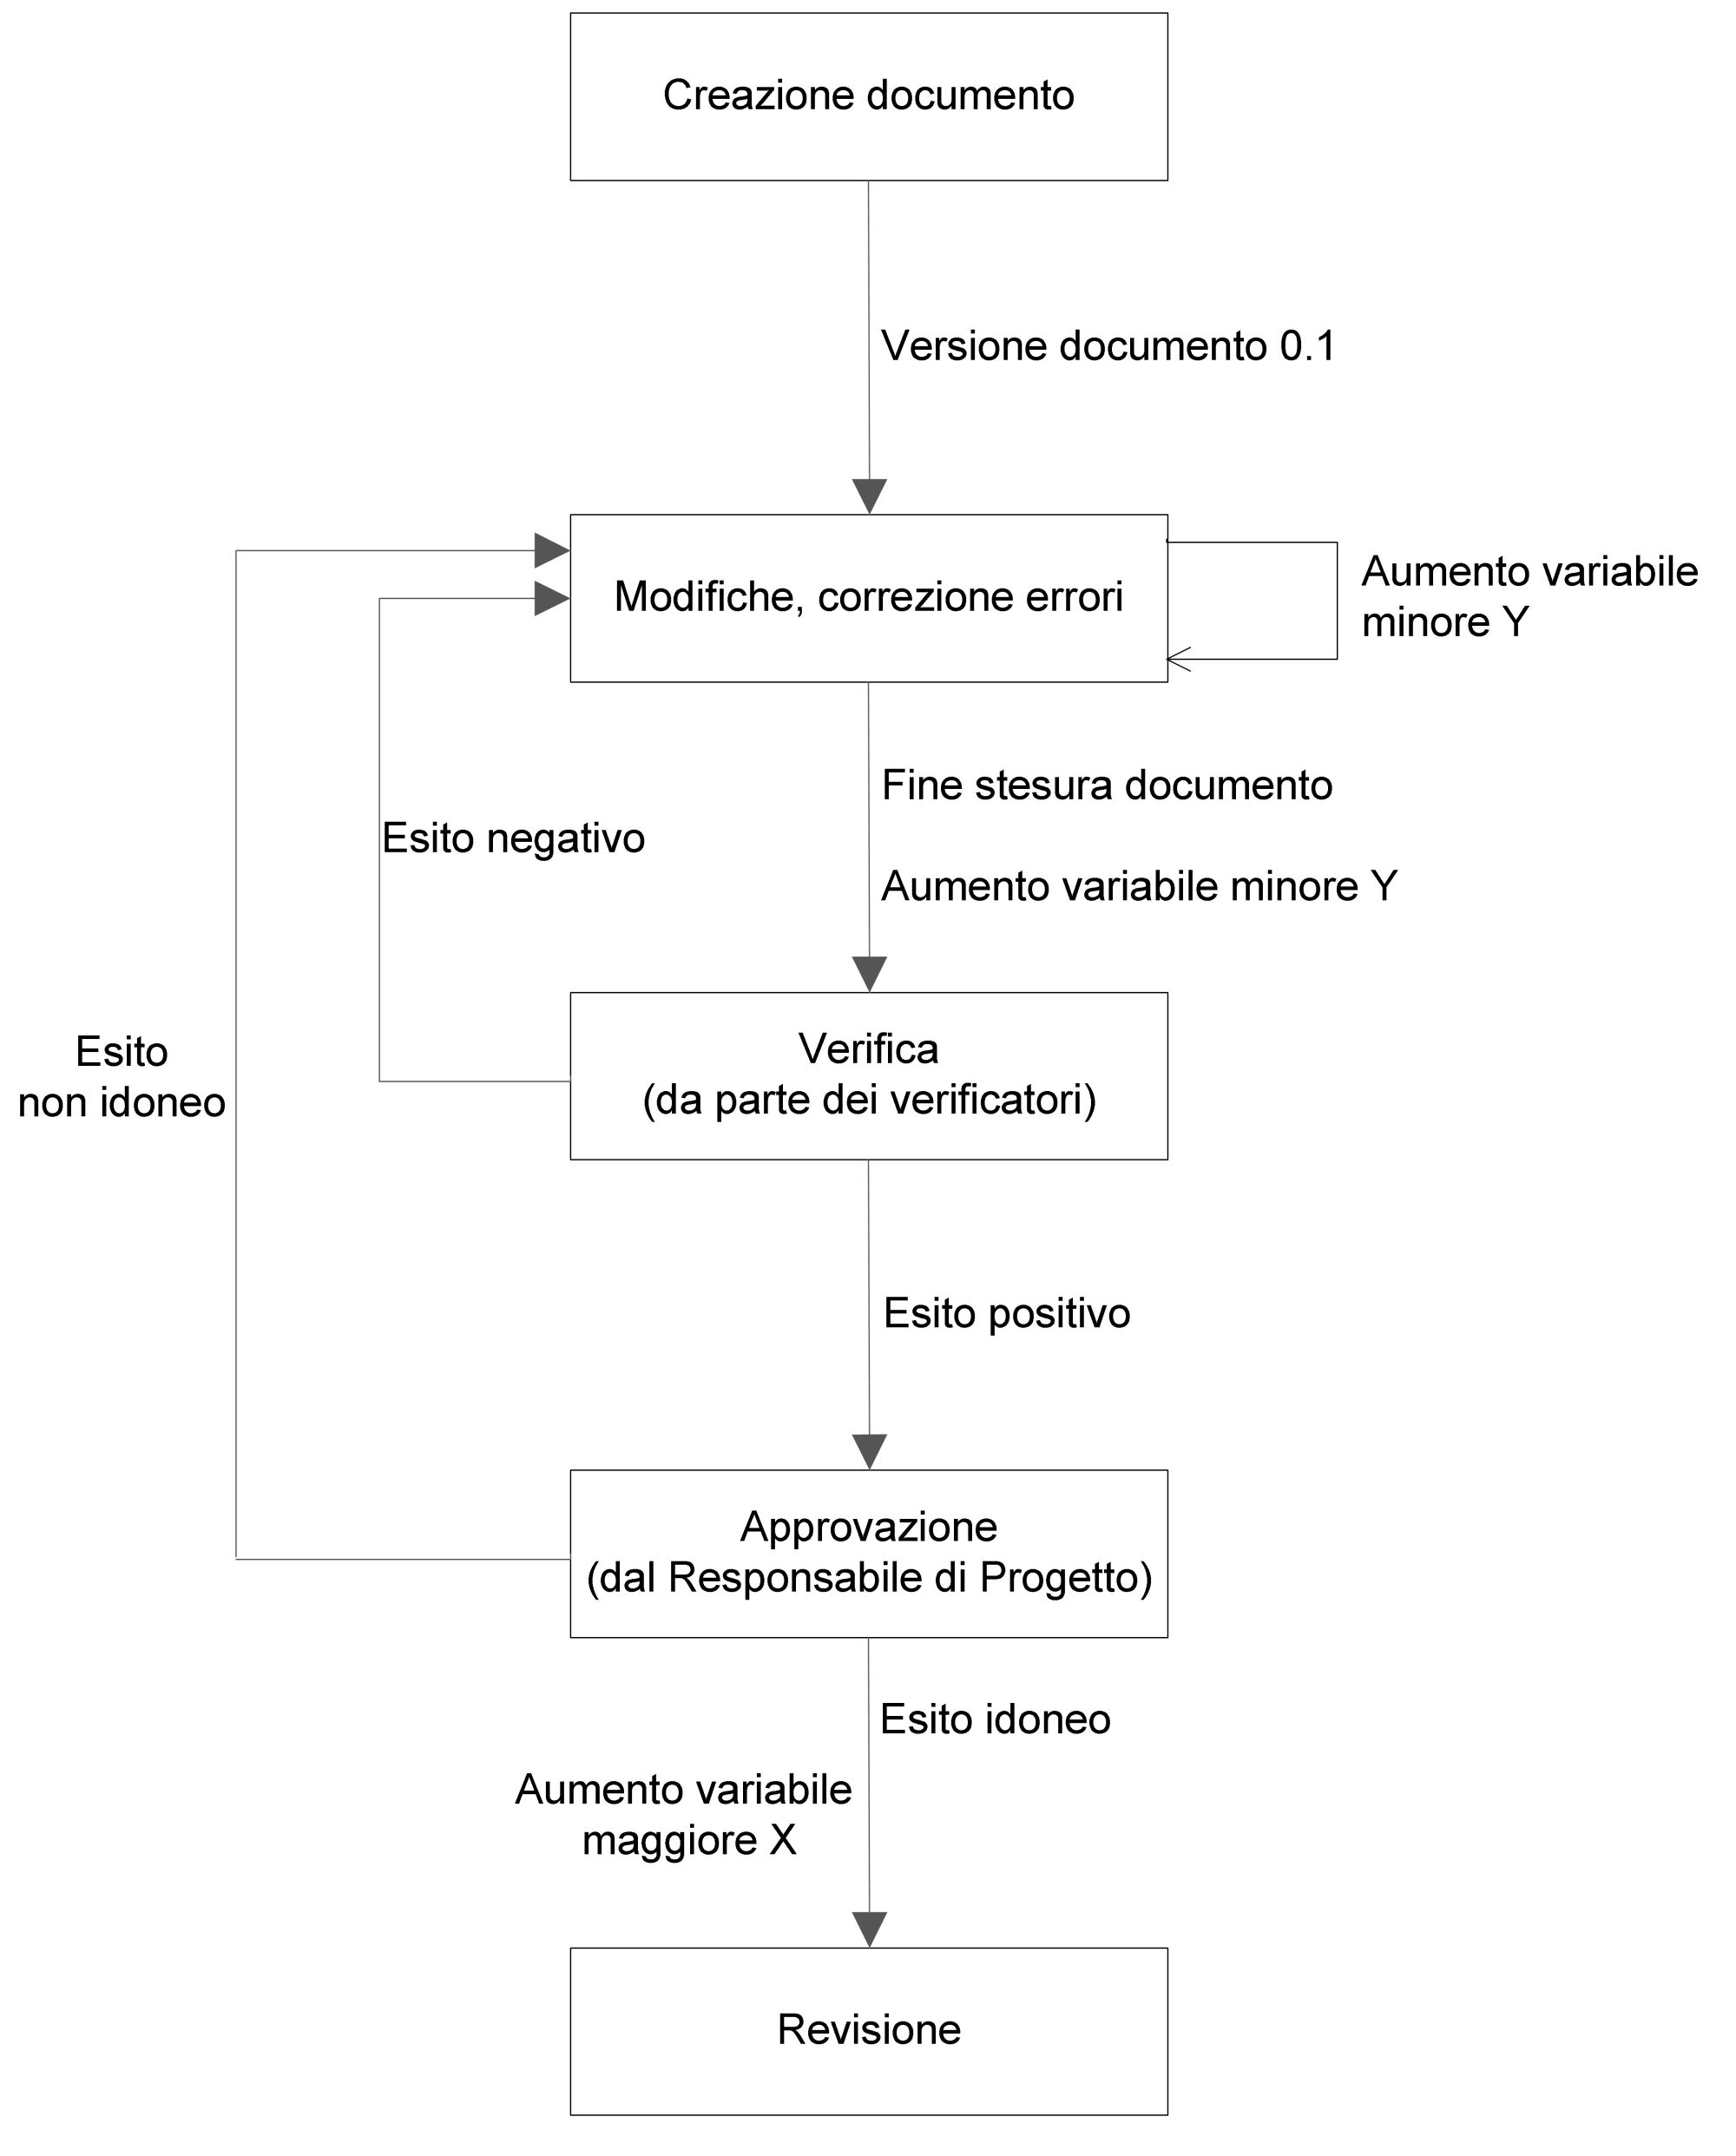
\includegraphics[scale=0.16]{ciclo_di_vita_documento}
\caption{Ciclo di vita di un documento} \label{fig:ciclo_di_vita_documento}
\end{figure}
\begin{enumerate}
\item Il redattore di un nuovo documento dovrà redigere in locale la prima impostazione del documento e solo allora potrà caricarlo nel \inglese{repository} secondo le regole indicate nelle sezione \ref{sec:repository} ``repository''.
\item Ad ogni sostanziale modifica verrà incrementato il contatore Y (vedi sezione \ref{sec:nomi_documenti} ``Nomi di documenti'') e seguirà un \inglese{commit} nel \inglese{repository}.
\item Quando il redattore finisce la stesura o revisione del documento, questo verrà proposto al verificatore il quale avrà il compito di controllare che siano state seguite le norme riguardanti la stesura di documenti (vedi sezione \ref{sec:verifica_documenti} ``Verifica dei documenti''). Il verificatore potrà dare due esiti, positivo o negativo.
\item In caso di esito negativo, il documento viene riproposto al redattore evidenziandone gli errori riscontrati. Se invece l'esito è positivo, il documento è stato redatto secondo le norme e non presenta errori, passerà quindi al responsabile di progetto che provvederà all'approvazione formale.
\item Anche il responsabile di progetto può dare due giudizi, idoneo o non idoneo. Nel caso di idoneità, il documento è da considerarsi formale e può essere inserito nella cartella corrispondente alla \inglese{milestone} presente nella directory \verb+Revisioni+.
\item In caso di non idoneità, il documento verrà rimandato al redattore notificando il motivo di tale decisione e si ripartirà dal punto 3.
\end{enumerate}

\subsection{Template}
Ogni documento dovrà essere generato includendo il \inglese{template} \LaTeX{} presente nella cartella \verb+Documents+.

Questo file è stato redatto prima dell'inizio di stesura di ogni altro documento sotto comune accordo. La modifica perciò di tale \inglese{template} deve essere richiesta all'amministratore di progetto che analizzerà l'esigenza e darà una risposta positiva o negativa.

In caso positivo, si procederà all'attuazione delle modifiche e verrà informato l'intero team al fine che ogni membro modifichi il documento su cui sta lavorando.

\subsection{Glossario}
Il glossario è un documento nel quale vengono riportate tutte le parole difficilmente comprensibili o dal significato ambiguo presenti nei documenti. È un documento un po' particolare in quanto non rispetta le regole stilistiche degli altri documenti.

Non sarà presente l'indice dei contenuti, ma solo una pagina iniziale contenente le informazioni del documento, la tabella delle modifiche, una breve introduzione e a seguire le voci ordinate alfabeticamente.

\subsection{Norme tipografiche}
Questa sezione descrive le norme da utilizzare per l'utilizzo dell'ortografia, tipografia e l'assunzione si uno stile uniforme nel redigere i documenti.

\subsubsection{Stili di testo}
\begin{itemize}
\item \textbf{Grassetto}: usato per evidenziare passaggi importanti. Si utilizza anche su elementi immediatamente seguenti agli elenchi per evidenziare l'oggetto trattato nel paragrafo.
\item \textbf{Corsivo}: usato per dare enfasi a parole o frasi su cui prestare attenzione, nonché per indicare i forestierismi (ad es.~i termini in inglese presenti in un documento).
\item \textbf{Sottolineato}: le parole sottolineate sono riportate nel glossario. Al fine di facilitare la lettura, nei documenti dovrà essere sottolineata solo la prima occorrenza di ciascun termine la cui definizione è riportata nel glossario.
\item \textbf{Maiuscolo}: deve essere utilizzato esclusivamente per sigle e acronimi.
\end{itemize}

\subsubsection{Punteggiatura}
Qualsiasi segno di punteggiatura non deve mai seguire uno spazio ma deve precederne uno. Dopo un punto fermo deve esserci uno spazio seguito da una lettera maiuscola.

Le parentesi vanno usate per raggruppare un periodo, non devono aprirsi con un carattere di spaziatura e non devono chiudersi con un carattere di punteggiatura o di spaziatura.

\subsubsection{Composizione del testo}
Gli elenchi, sia puntati che numerati, vanno usati per elencare una serie di elementi e solitamente hanno una breve lunghezza con la quale descrivono l'elemento in questione.

Per questo, ogni punto elenco deve finire con un punto e virgola (;) tranne l'ultimo elemento che finirà con un punto (.), mentre nel caso di punti elenco più discorsivi la frase finirà con un punto ogni volta.

Per quanto concerne le note a piè di pagina invece, ogni nota dovrà cominciare con la prima lettera della prima parola maiuscola, senza spaziatura davanti e finire con un punto.

\subsubsection{Formati ricorrenti}
\label{sec:formati_ricorrenti} 
\begin{itemize}
\item \textbf{Path}: per scrivere indirizzi web e url si adotterà il comando prestabilito da \LaTeX \verb+ \url+.
\item \textbf{Date}: per scrivere una data si dovrà utilizzare il formato AAAA-MM-GG (standard ISO 8601) dove:
\begin{itemize}
\item AAAA: sta ad indicare l'anno;
\item MM: sta ad indicare il mese;
\item GG: sta ad indicare il giorno.
\end{itemize}
\item \textbf{Sigle}: di seguito sono elencate una serie di sigle, da usare principalmente all'intero di diagrammi o tabelle per risparmiare spazio.
\begin{itemize}
\item AR: documento ``Analisi dei Requisiti''
\item PdP: documento ``Piano di Progetto''
\item PdQ: documento ``Piano di Qualifica''
\item NdP: documento ``Norme di Progetto''
\end{itemize}
\end{itemize}

\subsection{Immagini}\label{image}
Tutte le immagini utilizzate nei documenti devono avere estensione \verb+.png+. Nel caso l'immagine abbia una grande dimensione, va compressa con il formato \verb+.jpg+. Devono risiedere tutte nella cartella \verb+Documents/pics+.\footnote{%
Si veda \url{https://github.com/SoftwareSynthesis/SoftwareEngineeringProject/Documents/pics}.
}

Nel caso di immagini riguardanti diagrammi UML, si deve rispettare la seguente regola per il nome file:
\begin{center}
\textit{tipologia\{x1-x2-..-xn\}}
\end{center}
dove ``tipologia'' dovrà essere una di queste sigle:
\begin{itemize}
\item \textbf{UC}: diagrammi casi d'uso;
\item \textbf{DC}: diagrammi delle classi;
\item \textbf{DO}: diagrammi degli oggetti;
\item \textbf{DS}: diagrammi di sequenza;
\item \textbf{DA}: diagrammi di attività;
\item \textbf{DP}: diagrammi di package.
\end{itemize}
e ``x1-x2-..-xn'' rappresenteranno la numerazione gerarchica dei diagrammi, dove il numero più a sinistra rappresenta il padre e quelli più a destra i figli.

Nel caso di immagine generiche, il loro nome dovrà rispecchiare il contenuto di tale immagine.

\subsubsection{Inserimento immagini}
L'inserimento di immagini all'interno del documento verrà fatto tramite l'utilizzo del comando \verb+\begin{figure}+ e \verb+\includegraphics[parametri]{riferimento}+ dove:
\begin{itemize}
\item \textbf{parametri}: indica una serie di parametri da utilizzare per formattare al meglio l'immagine, come una scala di ridimensionamento (\verb+[scale=0.8]+ indica un ridimensionamento del 20\%), l'altezza e larghezza (\verb+[width=2cm, heigh=4cm]+ indica un'immagine larga 2 cm e alta 4 cm) oppure parametri del tipo \verb+[width=\textwidth]+ per indicare che la figura corrisponda esattamente alla larghezza del testo;
\item \textbf{riferimento}: va messo il nome dell'immagine presente nella cartella \verb+pics+ (vedi sezione \ref{sec:struttura}) che si vuole inserire.
\end{itemize}
Prima della chiusura (\verb+end{figure}+) vanno inseriti anche i comandi \verb+\caption{didascalia}+ e \verb+\label{riferimento}+ per permettere l'indicizzazione e l'identificazione delle immagini tramite un codice.

\subsection{Inserimento tabelle}
L'inserimento di tabelle all'interno dei documento verrà fatto tramite l'utilizzo del package tabularx che permette la creazione di colonne a larghezza dinamica.

Vanno inseriti prima della chiusura della tabella (quindi prima del comando \verb+\end{tabularx}+) i comandi \verb+\caption{didascalia}+ e \verb+\label{riferimento}+ per permettere l'indicizzazione e l'identificazione delle tabelle tramite un codice.

\subsection{Inserimento link}
L'inserimento di riferimenti ipertestuali a pagine web avviene mediante il comando 
\begin{center}
\verb+\url{+\textit{link ipertestuale}\verb+}+
\end{center}
dove con \textit{link ipertestuale} indica l'indirizzo nella forma estesa 
\begin{center}
\url{http://www.dominio./estensione/...}
\end{center}


\subsection{Verifica dei documenti}
\label{sec:verifica_documenti}
La verifica di un documento avviene nel momento in cui il redattore ha finito di redigere completamente il documento.

Tale \underline{processo} si articolerà principalmente in tre fasi:
\begin{enumerate}
\item Si procederà con un'analisi ortografica, compreso il corretto uso della punteggiatura, degli accenti e degli apostrofi. Per far ciò il verificatore potrà aiutarsi con lo strumento ``Verifica ortografia'' presente in TexMaker raggiungibile dalla scheda ``Modifica->Verifica Ortografia''. Successivamente controllerà l'assenza di errori grammaticali, logici e sintattici nei periodi ed infine la coerenza del documento con le norme previste nella sezione \ref{sec:ambiente_documentale} ``Ambiente documentale''.
\item Se è la prima volta che il documento viene verificato, il verificatore procederà con un metodo di tipo \inglese{walkthrough}, come descritto in sezione \ref{analisi_statica}. Se invece il documento era già stato verificato e rimandato per via di errori, si adopererà un metodo di tipo \inglese{inspection},come descritto in sezione \ref{analisi_statica}.
\item Il verificatore prenderà nota in modo ordinato di tutti gli errori riscontrati e procederà con la creazione dei \inglese{tickets} relativi che saranno rivolti al redattore del documento come descritto nella sezione \ref{sec:ciclo_vita_ticket} ``Ciclo di vita di un Ticket''.
\end{enumerate}

\clearpage
\section{Milestones e Ticketing}
Allo scopo di agevolare lo svolgimento delle operazioni di assegnazione dei lavori e revisione durante l'intero ciclo di vita del progetto, l'azienda \team{} userà il servizio Codebase. Questo permette la creazione di \inglese{milestone} e \underline{\inglese{tickets}}, strumenti molto utili per tracciare il lavoro del team e anche per delineare una \underline{roadmap} degli obiettivi a breve e lungo termine che l'azienda si prefigge di raggiungere.

\subsection{Milestones}
Come prima cosa, il responsabile di progetto dovrà inserire tutte le \inglese{milestone} previste dal progetto, ossia le quattro revisioni.
\subsubsection{Creazione nuova Milestone}
\label{sec:creazione_milestone}
Per inserire una nuova \inglese{milestone} ci si dovrà posizionare nella pagina web dedicata alle \inglese{milestone} e cliccare su ``New Milestone''.
\begin{figure}[h]
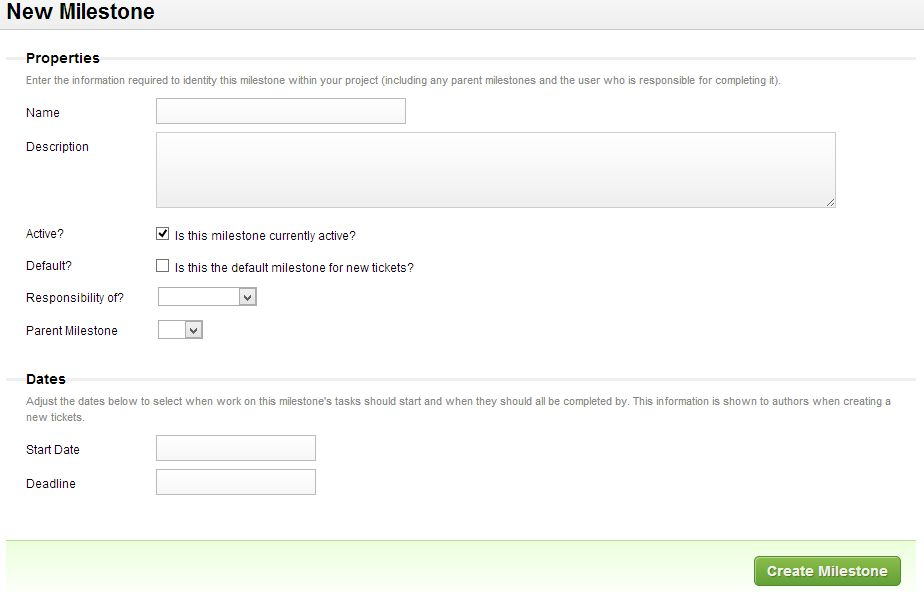
\includegraphics[width=\textwidth]{creazione_milestone}
\caption{Creazione di una nuova Milestone} \label{fig:creazione_milestone}
\end{figure}
Il form va completato nel seguente modo:
\begin{itemize}
\item \textbf{Name}: inserire il nome della \inglese{milestone};
\item \textbf{Description}: inserire una breve descrizione della \inglese{milestone};
\item \textbf{Active?}: flag da spuntare se si vuole che la \inglese{milestone} creata sia quella attiva;
\item \textbf{Default?}: flag da spuntare se si vuole che i futuri \inglese{tickets} creati siano riferiti a questa \inglese{milestone};
\item \textbf{Responsibility of?}: selezionare la persona responsabile;
\item \textbf{Parent \inglese{Milestone}}: selezionare se la \inglese{milestone} che si va a creare è figlia di qualche altra \inglese{milestone};
\item \textbf{Start Date}: inserire la data da cui far iniziare la \inglese{milestone};
\item \textbf{Deadline}: inserire la data di chiusura delle \inglese{milestone}.
\end{itemize}
Nel caso non si conosca qualche informazione, si può lasciare il relativo campo bianco e modificarlo successivamente (vedi paragrafo seguente) quando sarà resa pubblica l'informazione.

\subsubsection{Modifica Milestone}
Per modificare una \inglese{milestone}, ci si deve posizionare nella scheda ``Edit \inglese{milestone}''. Per raggiungerla, basta entrare nella \inglese{milestone} che si vuole modificare e cliccare sul bottone ``Edit \inglese{milestone}'' situato nella parte alta dello schermo a destra.
\begin{figure}[h]
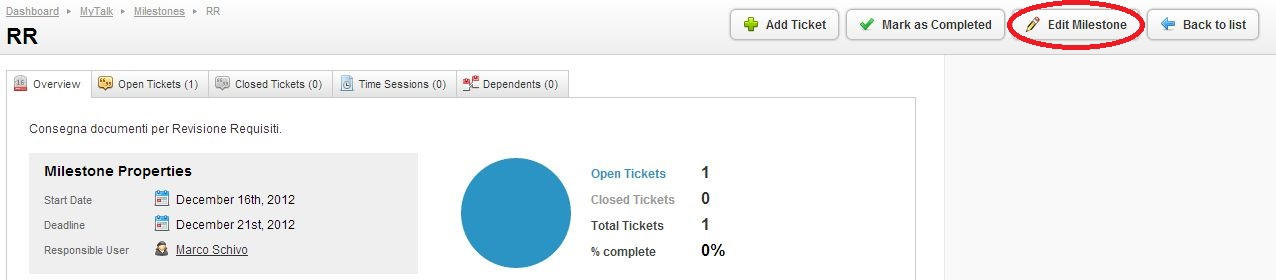
\includegraphics[width=\textwidth]{modifica_milestone}
\caption{Modifica di una Milestone} \label{fig:modifica_milestone}
\end{figure}
\\Per la compilazione dei campi, valgono le stesse regole riportate nella sezione \ref{sec:creazione_milestone} ``Creazione nuova \inglese{milestone}''.
\\Da notare che si può eliminare anche una \inglese{milestone} da tale scheda, basta cliccare sul bottone ``Delete Milestone'' presente nella parte destra della pagina.

\subsection{Ticketing}
Un \underline{ticket} rappresenta un compito da svolgere.

\subsubsection{Creazione nuovo Ticket}
\label{sec:creazione_ticket}
Per inserire un nuovo ticket ci si dovrà posizionare nella pagina web dedicata ai \inglese{tickets} e cliccare su ``New Ticket''.
\begin{figure}[h]
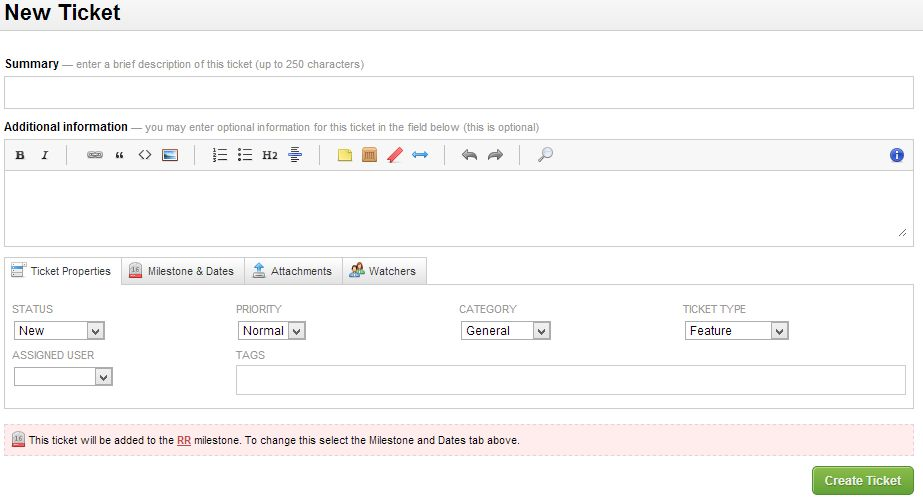
\includegraphics[width=\textwidth]{creazione_ticket}
\caption{Creazione di un nuovo Ticket} \label{fig:creazione_ticket}
\end{figure}
Il form va completato compilando obbligatoriamente i seguenti campi:
\begin{itemize}
\item \textbf{Summary}: inserire il nome del compito da assegnare;
\item \textbf{Status}: da impostare su ``New'';
\item \textbf{Priority}: selezionare la priorità effettiva del compito;
\item \textbf{Ticket Type}: da impostare su ``Task'';
\item \textbf{Assigned User}: selezionare la persona che dovrà svolgere il compito;
\item \textbf{Milestone}: selezionare la \inglese{milestone} corrispondente del compito.
\end{itemize}
Tutte le altre informazioni possono essere completate se si ritiene opportuno dare maggiori dettagli.

\subsubsection{Modifica Ticket}
Durante l'intero ciclo di vita di un ticket, questo viene modificato molte volte come avviene ad esempio quando dobbiamo modificare lo stato del ticket. Per far ciò, basta entrare nel ticket che si vuole modificare e appare subito la scheda di modifica.
\begin{figure}[h]
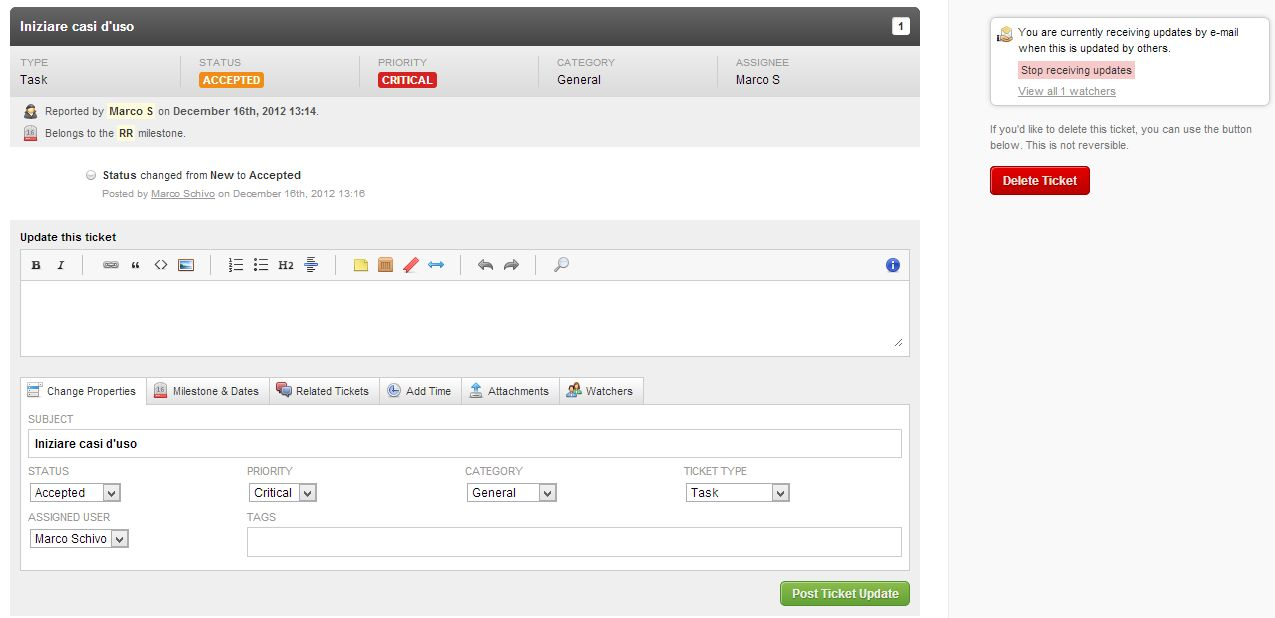
\includegraphics[width=\textwidth]{modifica_ticket}
\caption{Modifica di un ticket} \label{fig:modifica_ticket}
\end{figure}

\subsubsection{Ciclo di vita di un Ticket}
\label{sec:ciclo_vita_ticket}

\begin{figure}[h]
\centering
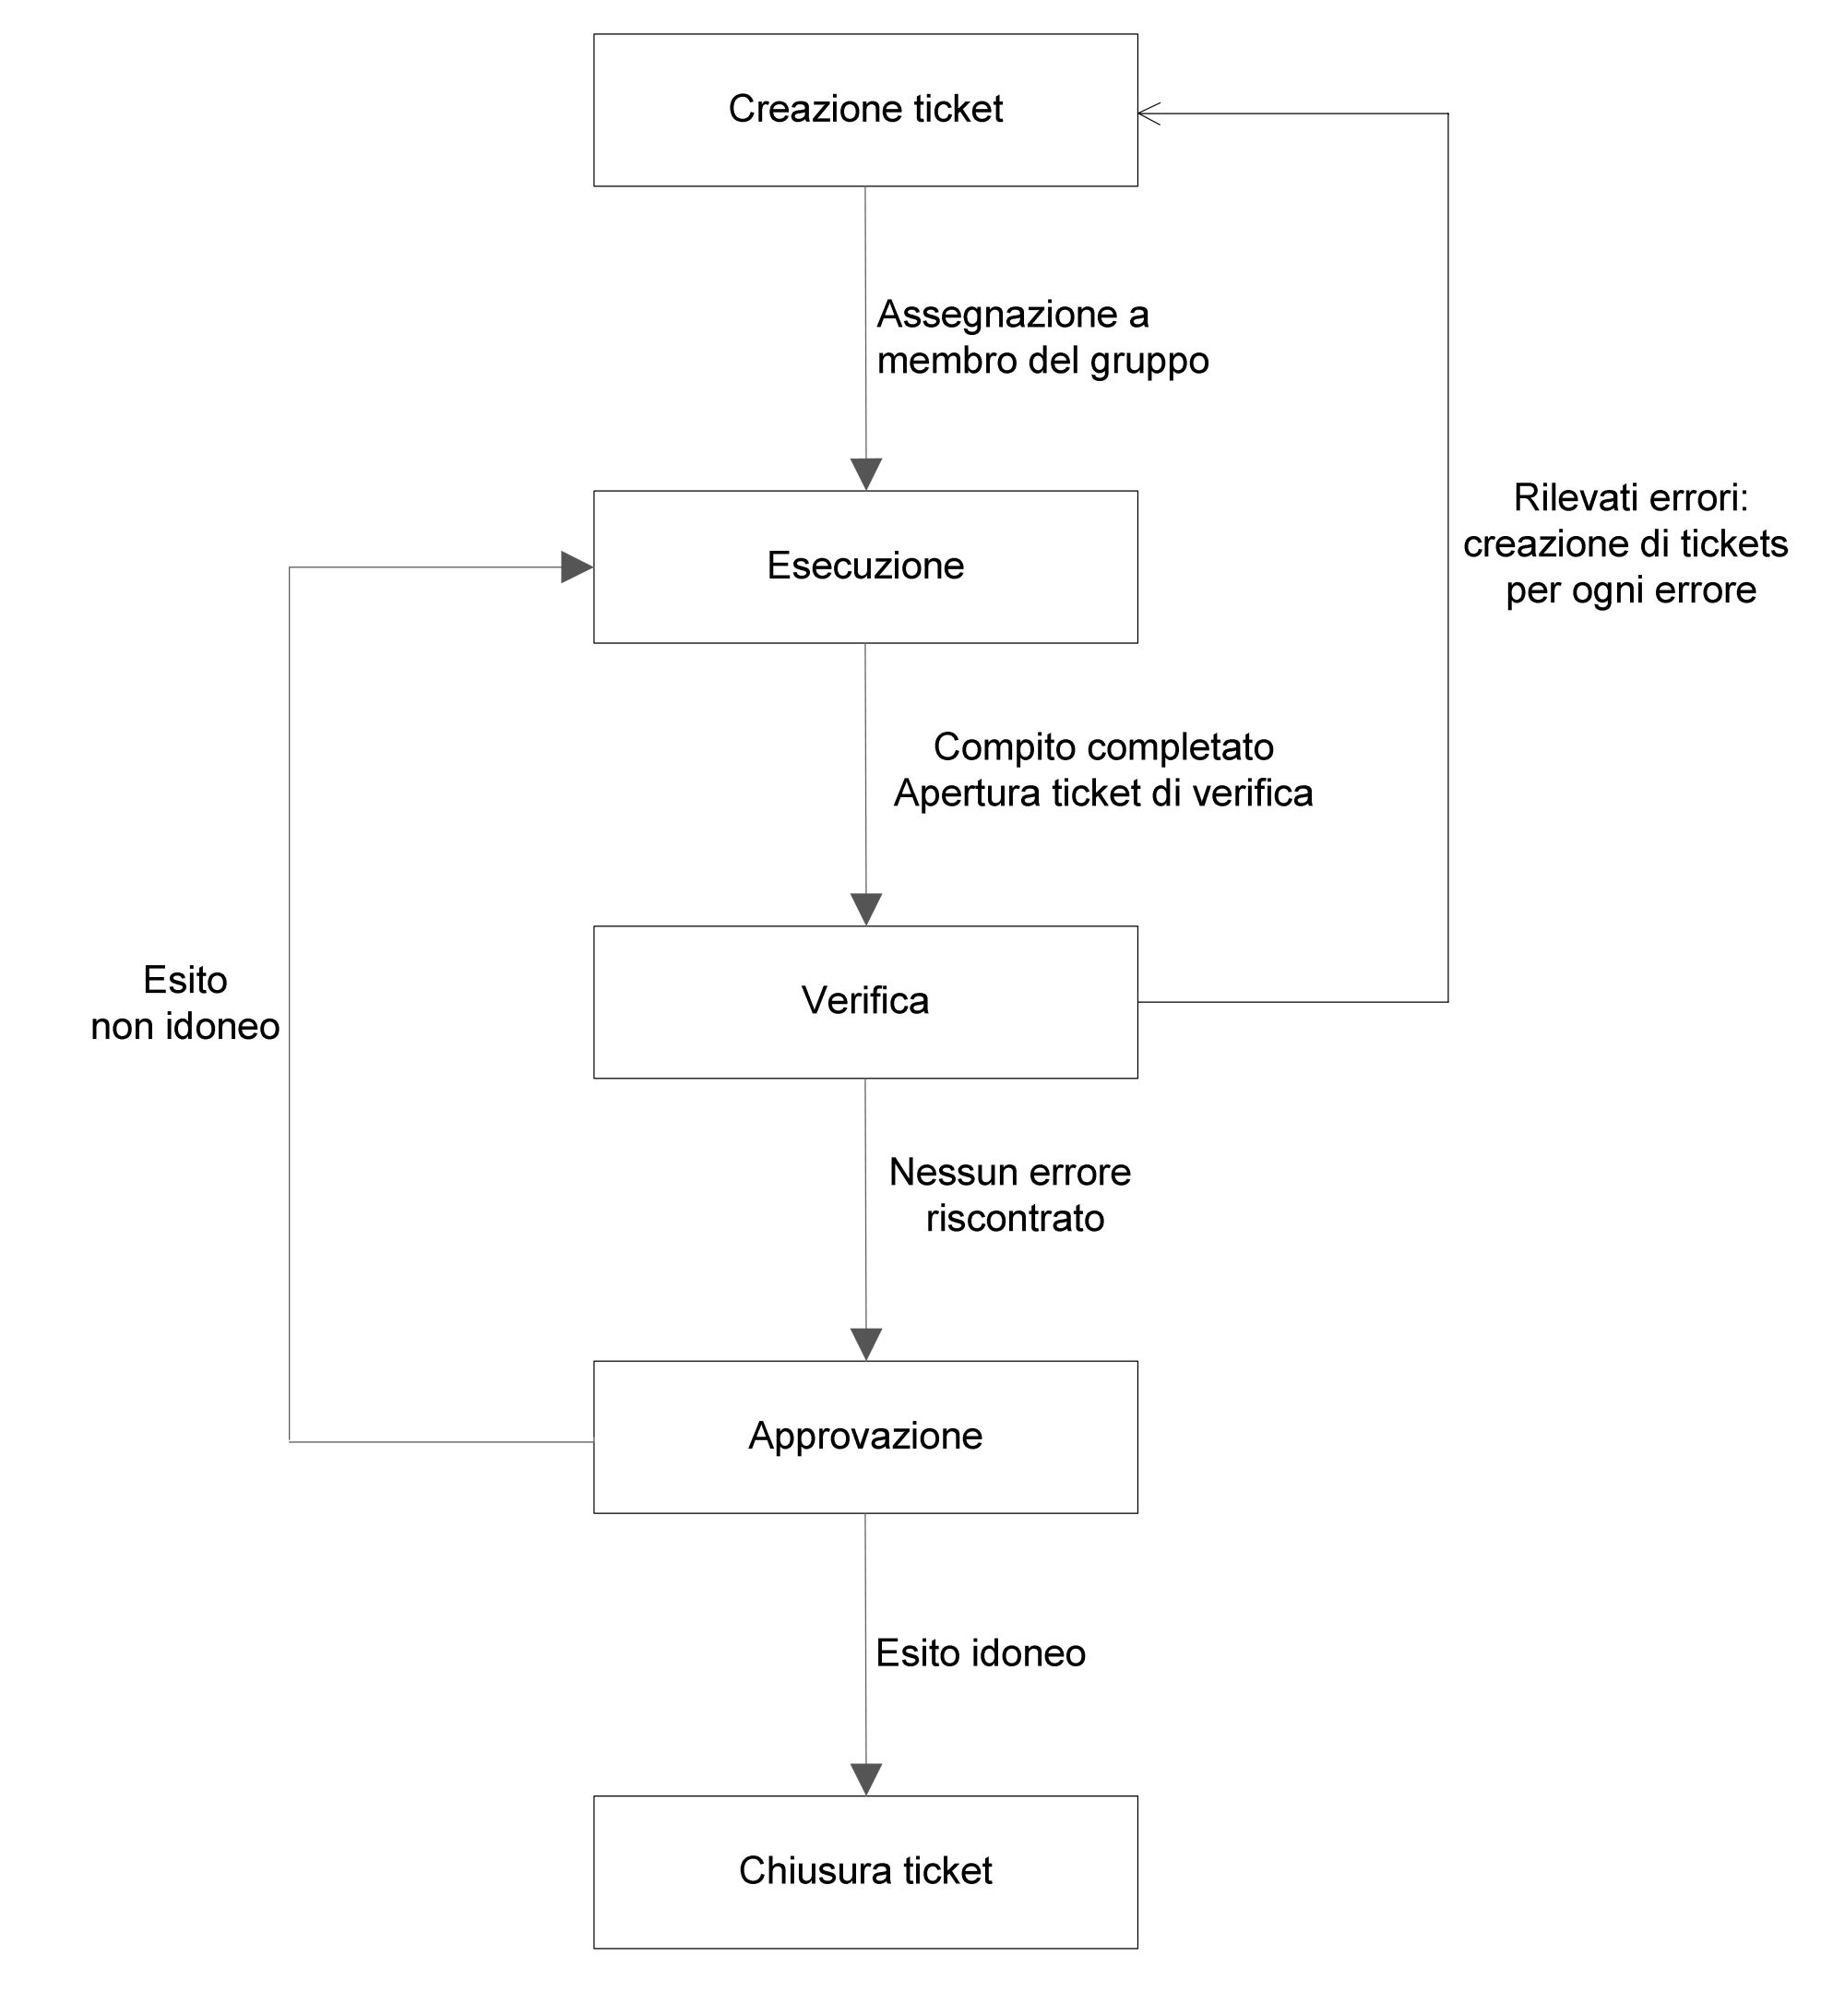
\includegraphics[scale=0.16]{ciclo_di_vita_ticket}
\caption{Ciclo di vita di un ticket} \label{fig:ciclo_di_vita_ticket}
\end{figure}
Come riportato in figura \ref{fig:ciclo_di_vita_ticket}, il ciclo di vita di un ticket si articolerà nel seguente modo:
\begin{enumerate}
\item \textbf{Creazione}: come prima cosa, il ticket va creato come descritto nella sezione \ref{sec:creazione_ticket} ``Creazione nuovo Ticket''.
\item \textbf{Esecuzione}: ogni membro dovrà prendere atto dei \inglese{tickets} a lui pervenuti e una volta visionati impostare lo stato ad ``\inglese{Accepted}'' o ad ``\inglese{Invalid}''. Una volta accettati, lo stato va modificato in ``\inglese{In Progress}'' quando si inizia a lavorarci e ``Completed'' quando si è portato a termine il compito assegnato.
\item \textbf{Verifica}: una volta che il compito è stato completato, si procede nella creazione di un nuovo ticket di tipo ``\inglese{Verification}'' il quale verrà assegnato ad un verificatore. Il nuovo ticket va compilato nel seguente modo:
\begin{itemize}
\item \textbf{Summary}: dovrà contenere il nome del documento o file da verificare;
\item \textbf{Status}: da impostare su ``\inglese{New}'';
\item \textbf{Priority}: selezionare la priorità effettiva del compito;
\item \textbf{Ticket Type}: da impostare su ``\inglese{Verification}'';
\item \textbf{Assigned User}: selezionare il verificatore che dovrà svolgere il compito;
\item \textbf{Milestone}: selezionare la \inglese{milestone} entro cui il documento dovrà essere verificato.
\end{itemize}
\item \textbf{Esecuzione verifica}: per ogni errore (esclusi quelli grammaticali) dovrà essere creato un nuovo ticket nel seguente modo:
\begin{itemize}
\item \textbf{Summary}: dovrà contenere il nome del documento o file da modificare;
\item \textbf{Additional information}: dovrà contenere la descrizione dell'errore presente nel documento;
\item \textbf{Status}: da impostare su ``\inglese{New}'';
\item \textbf{Priority}: selezionare la priorità effettiva del compito;
\item \textbf{Ticket Type}: da impostare su ``\inglese{Bug}'';
\item \textbf{Assigned User}: selezionare il Responsabile del progetto;
\item \textbf{Milestone}: selezionare la \inglese{milestone} entro cui il documento dovrà essere verificato.
\end{itemize}
Sarà  compito del Responsabile approvare o invalidare il ticket. In caso di non approvazione, il Responsabile dovrà decidere a chi far eseguire la modifica. Il membro selezionato dovrà quindi risolvere l'errore. Una volta completata la modifica il Responsabile dovrà riapplicare la procedura a partire dal punto 3.
\end{enumerate}
Quando tutti i \inglese{tickets} di una \inglese{milestone} avranno stato ``\inglese{Completed}'', significa che tutte le attività sono state svolte e il Responsabile potrà procedere alla chiusura della \inglese{milestone}.

\clearpage
\section{Analisi dei Requisiti}
L'analisi dei requisiti dovrà essere redatta dagli analisti. Il documento si presenterà suddiviso principalmente in tre parti: una prima parte riguardante i requisiti, una seconda parte riguardante i casi d'uso e la parte finale riguardante il tracciamento dei due elementi appena elencati.

\subsection{Norme per i requisiti}
La parte riguardante i requisiti dovrà elencare ordinatamente tutti i requisiti evinti dal capitolato d'appalto o dagli incontri con il proponente. Per far ciò, \textit{ogni requisito avrà nome univoco} e dovrà essere indicato nel formalismo:
\begin{center}
R\{Ambito\}\{Tipo\}\{Priorità\}\{Gerarchia\}
\end{center}
dove:
\begin{itemize}
\item \textbf{Ambito}: indicherà l'ambito del requisito e potrà assumere i seguenti valori
\begin{itemize}
\item U per indicare ``Utente'';
\item S per indicare ``di Sistema''.
\end{itemize}
\item \textbf{Tipologia}: indicherà il tipo del requisito e potrà assumere i seguenti valori:
\begin{itemize}
\item F per indicare ``Funzionale'', ossia requisiti che definiscono quali funzioni devono essere comprese. Tali requisiti si verificano per mezzo di test, dimostrazioni formali e revisioni.
\item Q per indicare ``di Qualità'', ossia definisce i requisiti sui fattori di rilievo della qualità, usabilità, sicurezza, scalabilità. Per questi deve essere adoperata una verifica ad hoc.
\item P per indicare ``Prestazionale'', ossia requisiti che stabiliscono vincoli su tempistiche e spazio, in relazione alla funzione da svolgere. Vengono verificati tramite misurazioni.
\item D per indicare ``Dichiarativo'', ossia requisiti con vincoli spesso ambientali e culturali. Si verificano per mezzo di revisione.

\end{itemize}
\item \textbf{Priorità}: indicherà la priorità del requisito e potrà assumere i seguenti valori
\begin{itemize}
\item O per indicare ``Obbligatorio'', ossia necessario per la realizzazione del progetto;
\item D per indicare ``Desiderabile'', ossia non obbligatorio ma, se implementato, aumenta il valore del progetto;
\item F per indicare ``Facoltativo'', ossia un requisito da implementare se avanzano risorse al termine del progetto.
\end{itemize}
\item \textbf{Gerarchia}: indicherà il grado di parentela dei requisiti e andrà specificato nella sintassi
\begin{center}
\textit{x.y.z}
\end{center}
dove il numero più a sinistra rappresenta il padre e quelli più a destra i figli.
\end{itemize}
Ogni requisito dovrà essere presente nel documento attraverso una ``scheda'', dove oltre i dettagli ricavabili dal nome, dovranno essere specificati anche una breve descrizione, la fonte (ossia la loro origine) e il motivo.\\\\
\textit{Esempio}\\
``RUFO2.3.1'' indica un requisito utente, funzionale obbligatorio con padre RUFO2.3.0 che a sua volta è figlio di RUFO2.0.0.

\subsection{Norme per i casi d'uso}
Il nome di ogni caso d'uso dovrà essere anch'esso, come per i requisiti, univoco e nella forma:
\begin{center}
UC\{n1.n2...n3\}
\end{center}
dove con ``{n1.n2...n3\}'' intendiamo la gerarchia, ossia il grado di parentela. Come per i requisiti, il numero più a sinistra rappresenta il padre e quelli più a destra i suoi figli.\\

\textit{Esempio}\\
``UC1.2.3'' indica un caso d'uso con padre UC1.2.0 che a sua volta è figlio di UC1.0.0.

\clearpage
Ogni caso d'uso al fine di essere descritto nel modo più esaustivo possibile conterrà i seguenti dettagli:
\begin{itemize}
\item \textbf{Nome}: composto dal codice di riferimento e una breve descrizione del caso d'uso;
\item \textbf{Descrizione grafica}: creata mediante il formalismo di UML e implementata tramite creazione di specifici casi d'uso per formalizzare e facilitare la comprensione del requisito;
\item \textbf{Descrizione didascalica}: viene correlata ad ogni diagramma di caso d'uso con una descrizione in cui compaiono le informazioni:
\begin{itemize}
\item Attori principali;
\item Scopo e descrizione;
\item Precondizione;
\item Postcondizione;
\item Illustrazione scenario principale;
\item Illustrazione scenario alternativo.
\end{itemize}
\end{itemize}
\subsection{Tracciamento}

\subsubsection{Casi d'Uso-Requisiti e viceversa}
Durante l'intero ciclo di vita del progetto, sono previste misure per il tracciamento dei casi d'uso con i relativi requisiti. Questo avviene grazie all'utilizzo del sistema di tracciamento dei requisiti ``\manager{}'' descritto nella sezione \ref{sec:tracciamento} ``Sistema di tracciamento dei requisiti''. Tutta la gestione è automatica e in output sarà visualizzata una tabella con tre colonne: Codice UC, Nome UC, Requisito. Questa soluzione facilita notevolmente la gestione di grandi quantità di dati e un notevole risparmio di tempo. Avviene anche la stampa inversa, ossia Requisiti-Casi d'Uso.

\subsubsection{Requisiti-Test}
È prevista anche una tabella che traccia i requisiti e relativi test da effettuare per verificare il soddisfacimento di tutti i requisiti. Tale tabella avrà tre colonne, la prima riporta il codice del requisito, la seconda il codice del test e nella terza colonna una breve descrizione del test da effettuare.
\clearpage

\section{Progettazione}\label{sec:progettazione}
Lo scopo principale di tale attività è di analizzare e produrre una visione generale del sistema garantendo solidità, efficienza e al tempo stesso il soddisfacimento dei requisiti emersi durante l'attività di analisi.
Il documento prodotto al termine di questa attività, la Specifica Tecnica, descriverà l'organizzazione generale dell'intero sistema prodotto, specificando le scelte architetturali in modo esauriente e giustificato. Si avranno inoltre definiti i vari test da da eseguire per verificare la correttezza d'interazione tra le varie parti del sistema stesso.\\

In questa sezione verranno descritte le specifiche che i progettisti dovranno seguire durante la loro attività di progettazione architetturale.

\subsection{Stile di progettazione}
Al fine di semplificare la futura fase di verifica, nonché la leggibilità degli schemi e diminuire il livello di rischio dovuto ad una progettazione errata, si dovranno rispettare le seguenti regole e linee guida:
\begin{itemize}
\item \textbf{Information hiding}: si dovrà seguire il principio di \inglese{information hiding}, ossia nascondere dettagli organizzativi tramite attributi e metodi privati e/o protetti in modo tale da ridurre la complessità del contratto della classe. Ciò aumenta il grado di protezione e abbassa il rischio di errori logici.
\item \textbf{Decomposizione}: dovrà essere eseguita una \textit{decomposizione modulare} al fine di identificare fin da subito i componenti terminali che non richiedono ulteriore scomposizione, in modo tale da abbattere tempi e costi già dalle prime fasi.
\item \textbf{Design pattern}: individuare i design pattern da poter usare e applicarli correttamente.
\item \textbf{Livello di dettaglio}: raggiungere un livello di dettaglio in modo da permettere la parallelizzazione della codifica e non lasciare decisioni ai programmatori. 

\item \textbf{Annidamento di chiamate}: non dovranno essere presenti nell'applicativo chiamate di metodi annidate con profondità maggiore di dieci. Se è necessaria una modifica di tale limite il progettista dovrà proporlo, con relativa giustificazione, al responsabile di progetto che valuterà la richiesta.
\item \textbf{Costrutti condizionali}: non dovranno essere presenti nell'applicativo flussi condizionali con profondità maggiore di cinque. Se è necessaria una modifica di tale limite il progettista dovrà proporlo, con relativa giustificazione, al responsabile di progetto che valuterà la richiesta.
\item \textbf{Ricorsione}: la tecnica di ricorsione dovrà essere evitata il più possibile. Nel caso venga utilizzata, il progettista dovrà giustificarne la scelta e fornire inoltre la correttezza per dimostrarne la terminazione.
\item \textbf{Parametri}: il numero di parametri passati ad una chiamata di metodo non dovrà superare il limite di sette.
\item \textbf{Concorrenza}: se vengono utilizzati flussi di esecuzione concorrenti, dovrà essere fornito anche il relativo diagramma di flusso.
\end{itemize}

\subsection{Design Pattern}
\label{sec:design_patterns}
Per ogni design \inglese{pattern} utilizzato, si dovrà dare una breve descrizione indicando:
\begin{itemize}
\item \textbf{Scopo}: verrà proposto lo scopo generico del pattern, al fine di evidenziare subito la sua utilità;
\item \textbf{Componenti che lo implementano}: verranno elencati i componenti dell'architettura di sistema, che implementano il \inglese{pattern} descritto. Per ogni componente verrà inoltre associato un diagramma esplicativo che ne rappresenta la struttura. In tale sezione saranno evidenziati i vantaggi derivanti dall'adozione del \inglese{pattern} nel particolare contesto di applicazione.
\end{itemize}

\subsection{Convenzioni sui diagrammi}
Si dovrà utilizzare il linguaggio UML per definire:
\begin{itemize}

\item \textbf{Diagrammi dei package}: dovranno essere presenti per la parte server implementata con Java. Servono per definire i \inglese{package}, ossia un raggruppamento di classi.

\item \textbf{Diagrammi delle classi}: Verranno usati per descrivere tipi di entità, le loro caratteristiche e le eventuali relazioni all'interno delle singole componenti.

\item \textbf{Diagrammi di attività}: dovranno essere presenti per mostrare generici flussi di attività che un utente può compiere all'interno dell'applicativo.

\item \textbf{Diagrammi di sequenza}: usati per definire le responsabilità dei vari package (o delle classi) nel portare a termine un determinato compito. Sarà necessario limitare la rappresentazione di cicli o percorsi alternativi ai soli casi per cui la loro omissione provochi difficoltà nella comprensione del funzionamento dell'applicativo. 
\end{itemize}

\subsection{Classi di verifica}
Si dovranno sviluppare, quando possibile, delle classi fittizie da utilizzare in fase di verifica e come prototipo.

\subsection{Tracciamento}
\label{sec:tracciamenti_progettazione}
Per il tracciamento generale di componenti, requisiti, classi, si utilizzeranno sei tabelle complessive con due colonne ognuna. Di seguito la lista di tali tabelle che devono comparire nel documento ``specifica tecnica'':
\begin{itemize}
\item requisiti-componenti;
\item componenti-requisiti;
\item componenti-design pattern
\item design pattern-componenti;
\item componenti-classi
\item classi-componenti.
\end{itemize} 
\subsection{Struttura della Specifica Tecnica}
Il documento relativo alla Specifica Tecnica sarà strutturato nel seguente modo:
\begin{itemize}
\item una breve introduzione che spiega lo scopo del documento, i formalismi adottati e i riferimenti alle norme;
\item un breve elenco degli strumenti utilizzati;
\item breve trattazione dei design pattern utilizzati seguendo le norme indicate nel paragrafo \ref{sec:design_patterns};
\item descrizione dell'architettura generale evidenziando i componenti rilevati in fase di progettazione indicando il tipo, la funzione e l'obbiettivo;
\item descrizione dell'architettura di dettaglio (quando disponibile);
\item diagrammi UML;
\item tracciamenti (come descritto in sezione \ref{sec:tracciamenti_progettazione}).
\end{itemize}

\section{Progettazione di dettaglio}
Lo scopo di questa attività è di descrivere in modo molto particolareggiato quello che dovrà essere il sistema, estendendo e specificando nel dettaglio quanto individuato nella specifica tecnica.

Al termine di tale attività si avrà a disposizione il documento \textit{Definizione di Prodotto}, contenente tutte le informazioni necessarie per la realizzazione pratica del sistema.

Così come nel caso della progettazione di alto livello il risultato dell'attività comprende altresì la definizione dei vari test da eseguirsi al fine di verificare la correttezza nel comportamento delle classi progettate.

I progettisti, analogamente a quanto stabilito relativamente all'attività precedente, dovranno attenersi più possibile alle specifiche elencate nei paragrafi seguenti.

\subsection{Diagrammi}
Come per la specifica tecnica si dovrà utilizzare il linguaggio UML per definire:

\begin{itemize}
\item \textit{diagrammi delle classi:} al fine di rendere più chiare ed esplicite possibili le relazioni tra le varie classi all'interno delle componenti;
\item \textit{diagrammi di attività:} per definire in modo univoco i flussi delle attività svolte dai vari componenti;
\item \textit{diagrammi di sequenza:} per definire in modo preciso le responsabilità dei package (o classi) nello svolgimento dei propri compiti. Come nel caso della specifica tecnica si dovrà limitare la rappresentazione di cicli o condizioni alternative ai soli casi in cui la loro presenza risulti necessaria alla comprensione del funzionamento dell'applicativo.
\end{itemize}

Tali diagrammi, ovviamente, hanno lo scopo di approfondire ove presenti quanto già descritto nel documento di specifica tecnica e possono pertanto essere trascurati nei casi in cui la loro specializzazione non porti alcun ulteriore beneficio alla documentazione.

\subsection{Specifica di una classe}
Al fine di garantire una rappresentazione più chiara e dettagliata di ogni classe all'interno del documento \textit{Definizione di Prodotto}, ogni classe dovrà essere descritta attenendosi al seguente schema:

\begin{itemize} 
\item \textbf{Funzione:} la funzione svolta dalla classe stessa.
\item \textbf{Relazione d'uso:} la relazione che la classe ha con altre classi (es. può \textit{estendere} o \textit{essere estesa}, \textit{implementare} o \textit{essere implementata}, da un altra classe, ecc.)
\item \textbf{Attributi:} gli attributi presenti all'interno della classe con una loro breve descrizione;
\item \textbf{Metodi:} i metodi (pubblici) che la classe possiede e una relativa descrizione comportamentale. Al fine di renderne più chiara la suddetta descrizione è consigliato descrivere anche le eventuali eccezioni che ciascun metodo può sollevare.
\end{itemize}

\subsection{Tracciamento}
Come nel caso della specifica tecnica sarà presente in forma tabellare il tracciamento di ogni requisito con le varie classi al fine di garantire la soddisfacibilità del medesimo, in modo che ogni classe ha ragione di esistere e non ne esista nessuna senza alcun ruolo all'interno del sistema creato.

\subsection{Struttura della Definizione di Prodotto}
Il documento relativo alla Definizione di Prodotto che estenderà ed integrerà quello di Specifica Tecnica conterrà:
\begin{itemize}
\item i diagrammi delle classi per ogni componente evedenziato;
\item le specifiche di \textit{tutte} le classi.
\end{itemize}

\subsection{Convenzioni di scrittura}
Al fine di rendere quanto più agevole possibile la consultazione di questo documento da parte dei programmatori e del committente, è stata adottata una serie di accorgimenti. In primo luogo, sono stati inseriti riferimenti incrociati sui nomi delle classi aventi come destinazione la sottosezione che descrive la classe stessa.

In secondo luogo, per i membri di classi e interfacce, oltre a una famiglia di font a spaziatura fissa, sono state adottate le seguenti convenzioni cromatiche:
\begin{itemize}[noitemsep,nolistsep]
\item \memberdata{\bfseries rosso} per i campi dati;
\item \method{\bfseries verde} per i metodi.
\end{itemize}
I differenti livelli di accessibilità sono contrassegnati, in maniera analoga a UML, come:
\begin{itemize}
  \item \texttt{\ttfamily +} per la parte pubblica;
  \item \texttt{\ttfamily \#} per la parte protetta;
  \item \texttt{\ttfamily \textasciitilde} per  l'accessibilità di package;
  \item \texttt{\ttfamily --} per la parte privata.
\end{itemize}

Infine, i membri statici di classi e interfacce sono contrassegnati con una \underline{\texttt{sottolineatura}}.

\clearpage
\section{Codifica}
Questa sezione andrà ampliata nel momento in cui si avvierà la vera attività di codifica. Vengono intanto fornite delle convenzioni di codifica generale.

\subsection{Intestazione dei file}
Tutti i file sorgente includeranno un'intestazione con le informazioni generiche relative al file medesimo quali:
\begin{itemize}[noitemsep,nolistsep]
\item[-] nome del progetto
\item[-] nome del team di sviluppo;
\item[-] nome del file;
\item[-] versione;
\item[-] data di creazione.
\end{itemize}

\subsection{Convenzioni di codifica}
Per rendere il codice più leggibile ed ordinato, per quanto riguarda l'uso del linguaggio Java, si dovranno rispettare le \textit{Java Code Convention}.\footnote{%
Disponibili all'indirizzo \url{http://www.oracle.com/technetwork/java/codeconvtoc-136057.html}.
}

Tali convenzioni di codifica possono essere variate, ma tale modifica deve essere richiesta al responsabile di progetto che valuterà la reale ed effettiva necessità di tale modifica.

\subsubsection{Convenzioni sui nomi}
\begin{itemize}
\item \textbf{Classi e Interfacce}: il loro nome è un sostantivo e deve avere la prima lettera maiuscola.
\item \textbf{Metodi}: devono avere il nome di un verbo e la prima lettera minuscola. Nel caso il nome sia composto da più parole, la prima lettera di ogni parola sarà maiuscola.
\item \textbf{Variabili}: devono avere un nome che ne rende chiaro immediatamente il significato. Nel caso il nome sia composto da più parole, la prima lettera di ogni parola sarà maiuscola.
\item \textbf{Costanti}: il nome va scritto tutto in maiuscolo. Nel caso il nome sia composto da più parole, vanno separate da un \inglese{underscore}.

\end{itemize}

\subsubsection{Struttura delle classi}
La classi dovranno essere composte riportando nel seguente ordine tali elementi:
\begin{enumerate}
\item variabili statiche e di istanza;
\item costruttori;
\item metodi.
\end{enumerate}

\subsubsection{Struttura del codice}
Per la stesura di codice, si seguiranno le seguenti regole:
\begin{enumerate}
\item le dichiarazioni di variabili andranno riportate tutte all'inizio e si dovrà usare una riga per ogni variabile;
\item ogni blocco di codice (tipo definizione di un metodo) va separato  con una linea bianca vuota;
\item le parentesi graffe che delineano un blocco di codice devono iniziare nella stessa riga della parola chiave a cui appartengono e finire in una nuova riga allineata con la parola d'inizio;
\item parole chiave e parentesi (ad esempio parentesi dovute a costrutti condizionali o ciclici) non devono essere separate da spazi.
\item l'annotazione \verb+@override+ sarà usata per assegnare automaticamente una descrizione definita per un metodo di una interfaccia/superclasse allo stesso metodo definito nella sottoclasse; serve inoltre al compilatore per controllare il corretto uso di \inglese{overloading} e \inglese{overriding};
\end{enumerate}

\subsection{Verifica del codice}
La verifica del codice verrà fatta, come prima cosa, durante lo sviluppo di ogni classe attraverso il proprio IDE che segnalerà gli errori più banali (errori di battitura o piccole mancanze).

Lo sviluppatore, prima di caricarlo nel \inglese{repository}, deve assicurarsi che il codice compili e non dia errori o \inglese{warning}.

Il verificatore successivamente dovrà assicurarsi che siano state rispettate le convenzioni descritte nella sezione \vref{sec:progettazione} e in caso di errori dovrà aprire un ticket (rispettando sempre le norme descritte in sezione \vref{sec:creazione_ticket}) rivolto allo sviluppatore che provvederà a risolvere gli errori.

\subsection{Norme sul codice Java}
Per la parte di progetto realizzato mediante codice java sarà usato Javadoc, un applicativo incluso nel Java Development Kit della Sun Microsystems, utilizzato per la generazione automatica della documentazione (in formato HTML) del codice sorgente scritto in linguaggio Java.

Il team ritiene pertanto che l'utilizzo di tale strumento sia non solo consigliato, ma bensì costituisca una \inglese{best practice}. I vantaggi che si prevede di ottenere utilizzando tale strumento sono:

\begin{itemize}
	\item imporre uno standard nella compilazione della documentazione dei sorgenti;
	\item facilitare il lavoro di documentazione che potrà (in parte) svolgersi in concomitanza con l'attività di programmazione (ossia nel momento in cui il programmatore è più focalizzato sull'argomento trattato);
	\item automatizzare l'esportazione dei documenti in due possibili formati: html e pdf.
	\item nel documentare si coglie anche il vantaggio di fornire commenti utili sul codice stesso, in grado quindi di aiutare i programmatori nelle future attività di programmazione.
\end{itemize}

Si vuole sottolineare che, al fine di garantire un formato più standardizzato possibile e quindi incline alla comprensione collettiva, le norme esposte successivamente saranno da applicare con la massima precisione.


I \textit{tag} Javadoc che verranno utilizzati sono i seguenti:
\begin{itemize}
\item \verb+@version+: numero di versione di una classe o di un metodo;
\item \verb+@author+: nome dello sviluppatore assegnato;
\item \verb+@param+: definisce i parametri di un metodo;
\item \verb+@return+: indica i valori di ritorno di un metodo (da non usare ovviamente nei metodi o costruttori con valori di ritorno \textit{void});
\item \verb+@throws+: indica le eccezioni lanciate da un determinato metodo;
\item \verb+@see+: indica un'associazione ad un altra classe o metodo.

\end{itemize}

Al fine di evitare la creazione di un tag Javadoc all'interno del codice in modo accidentale, sarà necessario utilizzare il codice HTML \&\#064, eliminando così ogni tipo di possibile ambiguità.

Definiamo in conclusione le convenzioni da utilizzare per la creazione di un commento Javadoc ben strutturato ed efficace :

\begin{itemize}
	\item è sempre posto subito prima della dichiarazione della classe, interfaccia, metodo, attributo.	
	\item è composto da due parti distinte: un tag e una descrizione. Deve iniziare con i caratteri \verb+/**+ e terminare con i caratteri \verb+*/+, ogni riga del commento dovrà inoltre iniziare con il carattere \verb+*+.
	\item avrà ragione d'esistere solo se la sua presenza sarà utile alla comprensione del codice, con un linguaggio sintetico, privo di ambiguità e più chiaro possibile.
	\item  è pensato allo scopo per descrivere le funzionalità o i principi di una unità (sia essa un package, una classe, un'interfaccia o un metodo) e non per ``spiegare'' pezzi di codice; tali commenti, anche se formattati secondo lo standard, non saranno mai estratti dal comando \texttt{javadoc};
	\item per ogni classe dovrà comprendere una descrizione delle sue funzioni, il tag \verb+@author+ con associato il nome dell'autore,il tag \verb+@version+ con il numero di versione di tale classe e la data di compilazione, infine il tag \verb+@return+ con il tipo di oggetto restituito.
	\item per ogni metodo, oltre ai tag già descritti e inseriti in una classe, dovrà contenere il tag \verb+@throws+ per ogni tipologia di eccezione che può sollevare e un tag \verb+@param+ per ogni parametro del metodo (con relativa descrizione).
\end{itemize}

\subsubsection{Manuale di Javadoc}

I programmatori del team di sviluppo possono inoltre avvalersi di ulteriori supporti per chiarire eventuali dubbi personali, come ad esempio al seguente link:
\begin{center}
\url{http://wwwusers.di.uniroma1.it/~parisi/Risorse/IntroJavadoc.pdf}
\end{center}

Qualora un membro del team trovasse eventuali informazioni che ritiene coerenti e di potenziale valore sarà suo dovere avvisare l'amministratore designato che vaglierà la possibilità di introdurle in questa sezione delle norme.

\subsection{Norme sul codice JavaScript}
In fase di codifica della parte JavaScript i programmatori dovranno fare in modo che il codice prodotto sia mantenuto in file con estensione \texttt{.js} separati rispetto alla parte \textit{html} e che in tutti i documenti \textit{html} che utilizzeranno tale codice sia inserito al loro interno, nel tag \inglese{head}, il riferimento al file JavaScript esterno.

Per quanto riguarda l'assegnazione del nome a variabili, funzioni e classi:
\begin{itemize}
\item il nome delle classi potrà essere composta da una o più parole: nel primo caso solo la prima lettera del nome sarà maiuscola, nel secondo caso le parole non dovranno essere separate, bensì verranno distinte dalla prima lettera (maiuscola) che le compongono (es: \texttt{AbilitaCanale});
\item il nome delle variabili sarà scritto utilizzando solamente lettere minuscole;
\item il nome delle funzioni come nel caso delle classi potrà essere composta da una o più parole, ma al contrario delle classi se composto ad una singola parola verrà scritta con caratteri esclusivamente minuscoli, se al contrario sarà composto da più parole verrà usata la convenzione scelta per le classi, ma la prima lettera (della prima parola) resterà minuscola;
\item il nome delle variabili, se composto da più parole, sarà creato dalle parole congiunte mediante \inglese{underscore}, dovranno inoltre essere utilizzate parole che identifichino il ruolo o lo scopo di tali variabili al fine di agevolare la comprensione del codice.
\end{itemize}

Infine, per quanto concerne le normative sul codice Javascript:
\begin{itemize}
\item al termine di ogni riga di codice dovrà esse presente il carattere ``;'' ;
\item in ogni funzione la prima parentesi dovrà essere posta a capo rispetto al nome e alla massima sinistra così come l'ultima parentesi (che identifica il termine del codice della funzione). 
\item il codice di ogni funzione sarà anticipato da una pre-condizione che ne spieghi concisamente lo scopo.
\item le parti di codice poco chiare o che fanno uso di funzioni specifiche dovranno essere correlate da commenti al fine di renderne comprensibile il funzionamento.
\end{itemize}

\clearpage
\section{Verifica e Validazione}
La verifica è un'attività molto importante svolta dal verificatore. Lo scopo è di accertare che i prodotti ottenuti, qualunque sia il loro tipo, siano conformi le norme e convenzioni riportate su questo documento.

Oltre a questo, il verificatore dovrà anche assicurare sotto la propria responsabilità che tali prodotti rispettino i requisiti di qualità descritti nel documento Piano di Qualifica (piano\_di\_qualifica.2.0.pdf).

\subsection{Strumenti di verifica}\label{sec:tools}
Si riporta a continuazione un elenco dei principali strumenti per la verifica di cui il team si dovrà avvalere nell'arco dello sviluppo del progetto.
\begin{itemize}
  \item \textbf{SynthesisRequirementManager}, il sistema di gestione dei requisiti (citato nel paragrafo \ref{sec:tracciamento} realizzato da \team, avente lo scopo di rendere quanto più agevole gestire il tracciamento dei requisiti a tutti i livelli (requisiti-UC, requisiti-CI, ecc.) e, da un punto di vista prettamente qualitativo, assicurare la necessità e la sufficienza dei casi d'uso e delle componenti software;
 \item \textbf{lacheck} ($\geq 1.26$) per assicurare la correttezza sintattica e l'adozione delle \inglese{best practices} per i sorgenti \LaTeX{} nonché rilevare in modo semi-automatico le sviste non segnalate dal compilatore in quanto pur corrispondendo a codice ben formato nascondono errori tipografici sottostanti per es.~bilanciamento delle virgolette, spaziature scorrette per frasi terminate da un acronimo prima di un punto, mancato utilizzo di spazi insecabili, ecc. (\url{www.ctan.org/pkg/lacheck});
 \item \textbf{hunspell} ($\geq 1.3$) come correttore ortografico e analizzatore morfologico in fase di redazione della documentazione, scelto per la sua portabilità ma anche perché alle sue librerie si appoggia l'applicativo \textbf{TexMaker} utilizzato per la stesura dei documenti \LaTeX{} (\url{http://hunspell.sourceforge.net});
 \item le utilità che costituiscono la suite di \underline{QA} del W3C al fine di verificare l'aderenza agli standard delle pagine web generate, in particolar modo gli strumenti online:
 \begin{itemize}
   \item \textbf{Unicorn} in qualità di strumento di validazione unificato (\url{http://validator.w3.org/unicorn});
   \item \textbf{CSS Valitatom Service} come utilità di validazione per i fogli di stile a cascata (\url{http://jigsaw.w3.org/css-validator});
 \end{itemize}
 \item gli strumenti per sviluppatori integrati in \textbf{Google \underline{Chrome}} (\url{https://developers.google.com/chrome-developer-tools}) e, in particolare:
   \begin{itemize}
   \item la sezione Sources che rappresenta un'interfaccia al \underline{\inglese{debugger}} per il motore \underline{JavaScript} V8 e consente di impostare \underline{\inglese{breakpoint}} (assoluti o condizionali) per seguire l'esecuzione del codice passo passo (con le consuete funzioni di \underline{``step over''}, \underline{``step into''} e \underline{``step out''}) nonché arrestare temporaneamente l'esecuzione al sollevamento di un'eccezione (o di un'eccezione non controllata);
   \item la sezione \inglese{Timeline} che permette di quantificare i tempi necessari al caricamento e all'esecuzione degli script, nonché di tracciare l'utilizzo della memoria e forzare l'invocazione del \inglese{garbage collector};
   \item  gli strumenti di benchmark accessibili dalla sezione \underline{Profiles}, vale a dire il \inglese{profiler} della CPU, che permette di ricostruire l'albero delle chiamate di funzione e la percentuale di utilizzo della CPU per ciascuna funzione, e il \inglese{profiler} dello \inglese{heap}, mediante il quale è possibile ispezionare il contenuto dello \inglese{heap} e salvarne delle rappresentazioni istantanee;
   \end{itemize}
  \item FirebugLite, un'estensione per Chrome che consente di ispezionare gli elementi \underline{HTML} e la struttura del DOM nonché di modificare in tempo reale i valori delle proprietà dei \underline{CSS} (\url{https://getfirebug.com/firebuglite});
  \item \textbf{SpeedTracer} uno strumento che consente di identificare i problemi di prestazioni nelle applicazioni web visualizzando una serie di metriche in tempo reale grazie all'analisi dei dati resi disponibili a livello di motore di rendering del \underline{browser} (\url{https://developers.google.com/web-toolkit/speedtracer});
  \item \textbf{JSLint} analizzatore statico di codice JavaScript volto a rilevare e impedire l'adozione inconsapevole di ``\underline{\inglese{worst practices}}'' in fase di codifica (\url{http://www.jslint.com});
  \item \textbf{ApacheBench} per testare l'efficienza prestazionale dell'applicazione lato server mediante la simulazione di un numero arbitrario di richieste da parte dei \underline{client} (\url{http://httpd.apache.org/docs/2.2/programs/ab.html});
  \item \textbf{Eclipse} \underline{IDE} multipiattaforma e \inglese{cross-language}, scelto in particolare come ambiente di sviluppo per la parte server da realizzarsi in \underline{Java}, che include al suo interno funzionalità di debugging (\url{http://www.eclipse.org}) utili ai fini della QA;
  \item \underline{plugin} \textbf{Metrics} per Eclipse, estensione che permette di associare un valore su una scala di riferimento al soddisfacimento di una serie di parametri di qualità del codice sorgente o metriche (\url{http://metrics.sourceforge.net});
  \item il plugin \textbf{FindBugs} per Eclipse, al fine di effettuare analisi statica del codice a livello di bytecode alla ricerca di potenziali cause di \underline{malfunzionamento} (\inglese{bug patterns}) o adozione inconsapevole di ``\inglese{worst practices}'' (\url{http://findbugs.sourceforge.net});
  \item \textbf{JUnit} come framework per i test di unità da effettuarsi relativamente alla parte server dell'applicazione (\url{http://www.junit.org});
  \item \textbf{QUnit} framework per i test di unità di codice \inglese{JavaScript}; 
  \item \textbf{JSCoverage}, \inglese{tool} per la misurazione del \inglese{Code Coverage} di codice \inglese{JavaScript}.;
  \item \textbf{eclemma}, \inglese{tool} per la misurazione del \inglese{Code Coverage} di codice \inglese{Java}. 

\end{itemize}

\subsection{Tecniche di verifica}
Responsabili delle attività di controllo interne al gruppo sono i verificatori, che si presuppone essere in ogni caso e senza alcuna deroga distinti dai realizzatori del prodotto soggetto a verifica (programmatori o redattori di documentazione). Al fine di garantire la qualità, i verificatori sono tenuti all'utilizzo di due tecniche di analisi: statica e dinamica.

\subsubsection{Analisi statica}
\label{analisi_statica}
L'analisi statica è un tipo di controllo basato sulla non esecuzione del codice, ma in senso lato può essere applicato a qualsiasi tipo di prodotto anche non propriamente eseguibile (ad es.~la documentazione di progetto).

Sono previste, in particolare, due forme di analisi statica: il controllo manuale (detto altrimenti ``\inglese{desk check}'') e il controllo assistito da strumenti automatici.

Per quanto concerne il \textbf{desk check}, cioè il controllo realizzato unicamente da parte di un agente umano, sono previsti due metodi formali:
\begin{itemize}
  \item \textbf{\underline{walkthrough}}: implica un esame ad ampio spettro del prodotto da verificare, che è preso in considerazione nella sua totalità in modo indiscriminato e senza alcuna assunzione previa sulla natura, la posizione e la frequenza degli errori da rilevare. Si tratta notoriamente di una tecnica molto onerosa in termini sia di tempo che di sforzo e può essere essa stessa per sua natura essere soggetta ad errori (in particolar modo falsi negativi). Tuttavia, almeno nelle fasi iniziali del lavoro, è l'unica scelta praticabile a causa della relativa inesperienza dei membri del gruppo nella realizzazione di prodotti complessi e articolati (sia software che documentazione). Allo scopo di ridurre il costo determinato dalla ripetizione di tale attività nell'arco di tutto il ciclo di vita è previsto che durante l'analisi in \inglese{walkthrough}sia stilata una lista di controllo relativa agli errori più frequenti e ai contesti in cui è più probabile che si producano errori in modo da collezionare una base di esperienza comune e consolidata destinata ad alimentare le attività di ispezione.
  \item \textbf{\underline{inspection}}: prevede un controllo mirato avente obiettivi specifici, ristretti e stabiliti a priori \emph{prima} che la verifica abbia luogo. Si tratta di un'attività meno dispendiosa in termini di risorse perché non presuppone l'analisi esaustiva del prodotto ma è focalizzata su determinate categorie di errori frequenti, enunciate in una lista di controllo (\inglese{checklist}) redatta sulla base dell'esperienza personale e delle attività di \inglese{walkthrough} precedentemente poste in essere.
\end{itemize}

La seconda forma di analisi statica prevede invece l'utilizzo di strumenti appositi denominati \textbf{analizzatori statici} e può essere svolta in modo semiautomatico senza richiedere necessariamente l'intervento di un umano. In particolare, come risulta dalla sezione \ref{sec:tools} si è stabilito di utilizzare degli analizzatori statici tanto per la parte documentale del progetto (come il comando \texttt{lacheck}) quanto per la parte propriamente eseguibile (JSLint per la parte JavaScript e FindBugs per la parte Java).

\subsubsection{Analisi dinamica}
I controlli dinamici, altrimenti definiti test, prevedono l'esecuzione del software in un ambiente controllato e con dati di input specificatamente pensati per testarne le funzionalità e l'aderenza ai requisiti mettendo in luce l'eventuale presenza di \underline{malfunzionamenti} dovuti alla presenza di \underline{difetti}. Caratteristica fondamentale dei test è la loro \emph{ripetibilità}, cioè dato lo stesso set di dati in ingresso e nello stesso contesto di esecuzione, l'output deve essere deterministico e univocamente determinato. Tale proprietà, unitamente all'auspicabile utilizzo di un \inglese{logger} che ha il compito di registrare le fasi dell'esecuzione del test, consente di individuare e riconoscere in maniera più agevole i difetti presenti nel prodotto.

In base al loro ambito di applicazione, i test possono essere suddivisi in:
\begin{itemize}
  \item test di unità aventi come oggetto le singole unità e, oltre al modulo da verificare e ai dati d'esempio, possono coinvolgere anche componenti attive (\inglese{\underline{driver}}) o passive (\inglese{\underline{stub}}) che siano in grado di simulare le parti del sistema non ancora disponibili al momento in cui il test viene eseguito;
  \item test di integrazione atti a verificare la corretta interazione e integrazione fra le componenti che costituiscono le parti del sistema e hanno come risultato una \inglese{build}, vale a dire un sottosistema funzionante che può essere eseguito in modo indipendente;
  \item test di sistema, volti a testare il rispetto dei requisiti software individuati in fase di analisi dei requisiti da parte dell'intero sistema; 
  \item test di regressione destinati a rilevare il caso indesiderabile in cui una modifica locale destabilizza il resto del sistema, si tratta del numero minimo di test necessario per scongiurare tale eventualità senza per questo dover ripetere \emph{in toto} i test di unità e di integrazione;
  \item test di accettazione, o collaudo, realizzato sotto la supervisione del committente per verificare l'aderenza del prodotto ai requisiti utente di più alto livello.
\end{itemize}

\subsection{Test di sistema e di unità}
La validazione dei test di sistema verrà svolta basandosi sui test specificati durante l'attività di analisi dei requisiti. I risultati di tali test verranno riportati in forma tabellare, in modo da renderne più pratica ed efficace la lettura e la comprensione.

L'esecuzione dei test avverrà mediante l'utilizzo di \textit{Selenium}, un \inglese{tool} che permette di impostare ed eseguire automaticamente i test per la dimostrazione delle funzionalità del sistema.

Per i test di unità al contrario la verifica dovrà basarsi sulle specifiche relative test di unità e di integrazione prodotte dalle attività di progettazione architetturale e di dettaglio, e verranno effettuati tramite i \textit{framework} Junit (per il codice java della parte server) e QUnit (per i test relativi al codice JavaScript).\\
Verrà successivamente redatto un documento riassuntivo contenente l'esito dei test in formato tabellare con specificati per ogni tipologia di test effettuati:
\begin{itemize}
\item ambiente in cui è stato svolto il test;
\item tipologia del test;
\item classi/Componenti testate nel test;
\item descrizione del test effettuato;
\item eventuali errori evidenziati dal test.
\end{itemize}

\subsubsection{JUnit e eclemma}
\textit{JUnit} è una libreria Java utilizzata per la creazione delle classi delegate ai test funzionali di metodi (o unità) di una determinata classe da analizzare, \textit{eclemma} invece ha il semplice scopo di calcolare il \textit{Coverage} del codice java scritto.
Per la creazione di tali test sarà necessario importare la libreria all'interno del progetto desiderato e successivamente creare un file che conterrà la classe con il codice effettivo del test.
All'interno di tale classe è possibile creare diversi metodi, che saranno preceduti dalle annotazioni proprie di \textit{JUnit}. Le più comuni sono:
\begin{itemize}
\item \textbf{@Test}: identifica i metodi utilizzati dalla classe per eseguire i test
\item \textbf{@Before} e \textbf{@After}: un metodo preceduto da tali annotazioni viene eseguito prima (o dopo) ogni esecuzione di un metodo contrassegnato da \textit{@Test}.
\item \textbf{@Beforeclass} e \textbf{@Afterclass}: il metodo viene eseguito solo una volta prima (o dopo) l'esecuzione della classe testata.
\end{itemize}
E' possibile inoltre creare classi ``suite'' che contengono più classi di test allo scopo di eseguirle in sequenza senza la necessità di avviarle singolarmente.\\\\
Concludiamo citando i metodi contraddistinti dal prefisso \textit{assert}, che hanno lo scopo di confrontare un valore preimpostato con il valore ritornato da un metodo restituendo \textit{true} o \textit{false} in base all'esito del test, risultando quindi molto utili per verificare la correttezza dello stesso.

\subsubsection{QUnit e JSCoverage}
Come accennato in precedenza, \textit{QUnit} è un framework per i test di unità del codice \inglese{JavaScript}. La sua esecuzione richiede una pagina \textit{HTML} all'interno della quale vengono inclusi i file \textit{qunit.js, css,js} e i file \textit{JavaScript} contenenti i test da eseguire.\\
Questi file dovranno riferire ad una specifica classe da testare e in particolare le funzioni ``test'', realizzae in modo da verificare che il valore di ritorno sia corretto (e quindi atteso) con specificate:
\begin{itemize}
\item una stringa che indica il compito della funzione;
\item la funzione che verrà richiamata all'avvio del test.
\end{itemize}

Le funzioni richiamate all'interno delle funzioni di \textit{test} sono offerte da \textit{QUnit} e specificano determinate azioni standard. 
Per una descrizione dettagliata di tali funzioni e del loro specifico compito si rimanda al sito di riferimento \url{http://docs.jquery.com/Qunit#Using_QUnit}.\\\\
\textit{JSCoverage} al contrario è un \inglese{tool} per valutare il {Code Coverage} integrabile con \textit{QUnit} in modo da ottenere contemporaneamente sia le informazioni relative al risultato dei test che quelle relative alla loro copertura in un unica pagina \textit{HTML} denominata \textit{jscoverage.html}.


\end{document}